\documentclass[12pt]{article}
\usepackage{fontspec}
\setmainfont{Times New Roman}
\XeTeXlinebreaklocale "ru"
\XeTeXlinebreakskip=0pt plus 1pt
\usepackage[margin=1in]{geometry}
\usepackage{amsmath,amssymb}
\usepackage{booktabs}
\usepackage{multirow}
\usepackage{graphicx}
\graphicspath{{../scripts/R/kz_passthrough/_outputs/}{../scripts/R/kz_valueadd/_outputs/}}
\usepackage[hidelinks]{hyperref}
\usepackage[authoryear]{natbib}
\usepackage{setspace}
\onehalfspacing
\usepackage{caption}
\captionsetup{font=small}

\title{Коридор, а не завод: переориентация торговли и отсутствующий\\
инвестиционный отклик в Казахстане, 2022--2025}

\author{Жанболат Какишев\thanks{Назарбаев Университет, \texttt{zhanbolat.kakishev@nu.edu.kz}.
\emph{Конфликт интересов.} Автор работает в Международном финансовом центре «Астана»
(AIFC), который управляет Международной биржей «Астана» и институционально связан с
государственными инвестиционными структурами Казахстана; ранее автор сотрудничал с
консалтинговой командой в рамках проекта по торговой стратегии Казахстана. Ни одна из
этих ролей не используется в эмпирическом анализе: он основан на публичных данных и на
коммерческих базах данных сделок, к которым автор имеет академический доступ.
В разделе~\ref{sec:policy} даются прямые рекомендации в области инвестиционной политики;
это личная позиция автора, сформированная с учётом, но не представляющая AIFC, QIC или
IFC. Приводимые здесь показатели инвестиционной деятельности государственного фонда взяты
из \citet{qicaifcifc2026pe} — отчёта, опубликованного совместно AIFC, QIC и IFC.
Материалы для воспроизведения результатов (код, спецификации запросов, публичные данные)
находятся в \texttt{scripts/R/kz\_passthrough/} и \texttt{scripts/R/kz\_valueadd/}.}}

\date{Сентябрь 2026}

\begin{document}
\maketitle

\begin{abstract}
\noindent Крупный, отраслевой по своему характеру рост спроса на торгуемый товар обычно
считается фактором, стимулирующим внутренние инвестиции. После февраля 2022 года, когда
прямая торговля России с её основными партнёрами оказалась нарушена, часть этой торговли
была переориентирована через соседние страны, включая Казахстан. Используя данные о
торговле на уровне товарных позиций (HS6, 2018--2025), мы измеряем этот шок спроса,
оцениваем, что удерживает Казахстан, и задаёмся вопросом, вызвал ли он инвестиции. Экспорт
в Россию по 29 товарным позициям резко возрастает начиная с мая 2022 года и увеличивается
примерно в десять раз (внешне составленный, не выбранный по этому результату приоритетный
список товаров вырос в 3.5$\times$ раза за тот же период); дата перелома устойчива к
HAC-коррекции, но разность разностей (DiD) по корзине не отделима от собственного правила
отбора корзины, а составленный извне приоритетный список из 50 позиций подтверждает дату
перелома и — на своих 26 неперекрывающихся позициях, при сопоставлении с «очищенной»
контрольной группой — эффект меньшей величины, так что идентификация опирается на даты
перелома, на абсолютные уровни и на сопоставление с соседними странами, а не только на
кросс-секционную регрессию. Перенос оптово-транспортной маржи (6--14\%, диапазон, который
мы выбираем, а не оцениваем) через таблицу «затраты--выпуск» даёт внутреннюю добавленную
стоимость в размере 5--11 центов на каждый переориентированный доллар против примерно
трёх четвертей на произведённый доллар — соотношение, которое сохраняется при любой марже
ниже примерно одной пятой. По данным трёх коммерческих баз данных о сделках мы не находим
инвестиционного отклика в секторах, через которые проходит поток, хотя четыре
пост-2022-х года позволяют исключить лишь крупный отклик. Мы интерпретируем это отсутствие
отклика через три «шлюза» --- доступ к рынку, необратимость и институты рынка капитала.
Крайняя конфигурация необратимости или рынок капитала, неспособный профинансировать
проходящие отбор проекты, каждый по отдельности снижают отклик до нуля; открытый шлюз
доступа к рынку делает это лишь совместно с малой маржой трансформации, а не сам по себе.
Кейс фиксирует открытый шлюз доступа к рынку, созданный таможенным союзом, который делает
торговлю близким заменителем производства, вместе с наводящим (но не доказательным)
свидетельством в пользу этой малой маржи, и показывает, что наименее ограниченный по
капиталу инвестор в экономике также не стал строить производство; связывает ли шлюз
необратимости самостоятельно, здесь установить нельзя. Казахстан функционирует как
коридор, а не как завод.

\medskip
\noindent\textbf{Ключевые слова:} переориентация торговли, шоки спроса, инвестиции в
условиях неопределённости, необратимость, промышленная политика, добавленная стоимость,
институциональные пустоты, транзитные экономики, Казахстан.
\quad\textbf{JEL:} F14, F15, E22, D25, O14, O24, O33, P33.
\end{abstract}

\clearpage

\section{Введение}

Когда спрос на торгуемую продукцию страны резко и устойчиво растёт, учебная логика
предполагает, что предложение последует за ним: фирмы расширяются, появляются новые
участники рынка, и если страна ранее импортировала данный товар, часть спроса начинает
удовлетворяться внутренним производством. Эта логика лежит в основе значительной части
экономики развития — от аргументов о защите молодых отраслей и импортозамещении до
современных работ о встраивании в глобальные цепочки создания стоимости и об
инвестиционных эффектах торговых шоков. Её предпосылка состоит в том, что достаточно
чёткий и достаточно устойчивый сигнал спроса рано или поздно вызывает инвестиционную
реакцию.

После февраля 2022 года Казахстан получил необычно «чистую» версию такого сигнала.
Нарушение прямой торговли между Россией и её основными партнёрами привело к
переориентации ряда торговых потоков через третьи страны. \citet{chupilkin2026roundabout}
документируют этот паттерн: резкое падение экспорта ЕС в Россию сопровождалось
соответствующим ростом экспорта ЕС в Армению, Казахстан и Кыргызскую Республику, с
подтверждением на уровне товарных позиций и зеркальной статистики роста экспорта этих
стран в Россию; \citet{chupilkin2025intermediated} количественно оценивают это замещение.
Та же переориентация документирована в политической литературе
\citep{simola2023bofit,kse2024exportcontrols,wisniewska2025osw}. Для Казахстана
переориентация сконцентрирована в чётко определённом наборе технологически ёмких товаров
и является крупной: на месячном уровне экспорт в Россию по этим позициям вырос примерно в
десять раз (в 3.5$\times$ раза — по составленному извне, не выбранному по этому
результату приоритетному списку; раздел~\ref{sec:shock}). Маршруты, спрос и товары
полностью наблюдаемы в торговых данных. Мы рассматриваем это как кейс-стади (крупный,
отраслевой, хорошо идентифицированный шок спроса) и задаёмся вопросом, вызвал ли он
внутренний инвестиционный отклик, который предсказывает учебная модель.

Мы действуем в три этапа.

\emph{Во-первых, мы измеряем шок.} Используя данные UN Comtrade на уровне HS6, годовые за
2018--2025 годы и месячные за 2019--2025 годы, мы выделяем из данных «корзину всплеска» из
29 товарных позиций, в которых отток в Россию и приток (от западных стран-респондентов и
Китая) как минимум удвоились с 2019--2021 годов по 2022--2024 годы. Агрегированный
исходящий поток резко переламывается в мае 2022 года (месячная статистика sup-$F$ равна
561, или 326 после коррекции Ньюи--Уэста, с неизменным доверительным интервалом); входящий
поток переламывается в том же месяце, но слабее, и вовсе не переламывается в более шумном
годовом ряде, где доминирует крупный, уже существовавший ранее поток из Китая. Армения и
Турция показывают тот же перелом 2022 года, а Кыргызская Республика и Грузия показывают
повышенный экспорт начиная с 2022 года на более шумном ряде — и всё это без сопоставимой
внутренней реформы (Приложение~\ref{app:breaks}). Разность разностей относительно
контрольных позиций даёт $\gamma = 2.44$ по выбранной на основе данных корзине, однако
перестановочный тест, согласованный с правилом отбора, помещает эту оценку внутрь
собственного нулевого распределения, поэтому мы не рассматриваем этот коэффициент как
идентифицированную величину эффекта. Составленный извне приоритетный список переламывается
в ту же дату и даёт частичное подтверждение эффекта меньшей величины: собственный рост
уровня по этому списку втрое меньше (3.5$\times$ против 11.6$\times$ у корзины всплеска), а
26 позиций приоритетного списка, не входящих в корзину всплеска, — при сопоставлении с
контрольной группой, очищенной от самой корзины всплеска, — показывают меньший, но
статистически различимый рост исходящего потока в Россию ($\gamma = 1.94$,
wild-cluster-бутстрап $p = 0.035$; собственный рост уровня 2.4$\times$; совместный
предтрендовый тест Вальда $F = 0.75$, $p = 0.528$), хотя не по входящему потоку
($\gamma = 1.12$, $p = 0.238$). Более крупный коэффициент приоритетного списка,
опирающийся на общие с корзиной всплеска позиции, не является артефактом одних лишь 24
общих позиций, но и его величина не является независимой от корзины всплеска: остаточные
позиции движутся в том же направлении, но с меньшей амплитудой. Плацебо-тест на крупнейших
гражданских позициях даёт обратный результат, при этом позиции, которым присвоено фиктивное
«лечение», не пересекаются с корзиной всплеска.

\emph{Во-вторых, мы измеряем, что удерживает Казахстан.} По приростному потоку в Россию
(около \$479 млн за 2022--2025 годы) данные об удельной стоимости и весе не позволяют чётко
отделить реэкспортный поток от обычной казахстанской торговли. Перенос
оптово-транспортной маржи (6--14\%, диапазон, который мы выбираем, а не оцениваем) через
таблицу «затраты--выпуск» (OECD ICIO) даёт внутреннюю добавленную стоимость около
\textbf{5--11 центов} на переориентированный доллар против примерно трёх четвертей на
доллар внутреннего промышленного производства. Поскольку шаг «затраты--выпуск» почти не
влияет на результат, итоговая цифра масштабируется пропорционально марже: она остаётся
ниже одной пятой произведённого доллара при любой марже ниже одной пятой
(раздел~\ref{sec:capture}). Таможенная пошлина на приростный поток составляет существенно
менее 1\% таможенных доходов, а валовой переориентированный поток — 0.2--0.3\% ВВП в год.

\emph{В-третьих, мы задаёмся вопросом, вызвал ли шок инвестиции.} Мы не находим отклика,
который можно было бы обнаружить в данных. Мы собираем данные на уровне сделок по слияниям,
поглощениям и сделкам прямых и венчурных инвестиций в Казахстане за 2015--2025 годы из трёх
коммерческих баз данных (Capital~IQ, PitchBook, Preqin), а также данные об агрегированной
инвестиционной деятельности государственной инвестиционной корпорации Казахстана, как это
отражено в \citet{qicaifcifc2026pe}. Заключение сделок в обрабатывающей промышленности
торгуемых товаров, транспорте и логистике, а также в дистрибуции происходит примерно с той
же интенсивностью, что и до 2022 года, если не ниже; при четырёх пост-2022-х годах тест
позволяет исключить лишь крупный отклик, а не умеренный сдвиг, и в любом случае это
отсутствие отклика переопределено: беспорядки января 2022 года, трансграничные
комплаенс-риски и репутационные издержки, присущие сделкам такого рода, а также волна
национализаций — каждый из этих факторов сам по себе снижал бы число сделок. Заявленная
стоимость сделок растёт, но концентрируется в передаче собственности на существующие или
проблемные активы (две из крупнейших сделок — национализации), тогда как гринфилд-проекты
и сделки по созданию новых мощностей не показывают роста после 2022 года.

Мы интерпретируем отсутствие отклика через рамку, в которой инвестиционный отклик является
произведением трёх «шлюзов»: \emph{необратимости} (станет ли кто-либо строить мощности под
столь неопределённый и зависящий от политики шок, имея возможность удовлетворить спрос
через торговлю?), \emph{доступа к рынку} (требуется ли внутренняя трансформация для выхода
на конечный рынок?) и \emph{институтов} (могут ли быть профинансированы проекты, прошедшие
первые два фильтра?). Для Казахстана шлюз доступа к рынку однозначно открыт (таможенный
союз со страной назначения делает торговлю близким заменителем производства), что близко к
достаточному условию нулевого отклика лишь совместно с малой маржой трансформации, а не
само по себе (раздел~\ref{sec:framework}), и это также означает, что Казахстан упускает
передачу технологий, которую вынудил бы режим правил происхождения
\citep{desouza2024diffusion}. Кейс также несовместим с институтами рынка капитала как
связывающим ограничением именно для этого нулевого отклика: государственная инвестиционная
корпорация, не испытывающая ни ограничений внешнего финансирования, ни проблем с выходом из
инвестиций, также не стала строить мощности под эту переориентацию. Связывает ли шлюз
необратимости \emph{самостоятельно} — здесь установить нельзя: внутристрановое сопоставление
(отклик сборочных производств на устойчивый шок спроса на легковые автомобили при
отсутствии отклика на реэкспортный шок) наводит на мысль, но осложнено смешением факторов, а
поскольку реэкспортный поток фактически сохранялся вплоть до 2025 года, участник рынка,
принимающий решение в 2022 году, сталкивался с неопределённостью относительно
продолжительности шока, а не с уже наблюдаемым краткосрочным явлением. Институциональный
шлюз объясняет отдельный факт: почему смежные устойчивые возможности, которые раскрывает
шок, остаются нефинансируемыми частным капиталом.

\paragraph{Вклад работы.} Работа вносит три вклада. (i) Основной вклад — эмпирический: насколько
нам известно, это первый анализ со стороны принимающей экономики того, что удерживает
транзитная экономика от переориентации торговли после 2022 года и вызвала ли она
инвестиции; работа расширяет литературу, устанавливающую факт и масштаб переориентации, до
вопроса о том, что удерживает от неё посредник, и продлевает горизонт анализа до 2025 года.
Работа также связана с результатом \citet{bowncrowley2007} о том, что
торгово-ограничительная политика отклоняет экспорт третьей страны на другие рынки:
настоящий кейс берёт этот отклонённый поток за отправную точку и задаётся вопросом, что
принимающая экономика с ним делает. Показано, что крупный, отраслевой шок спроса на
торгуемый товар не породил заметного инвестиционного отклика — факт, который говорит о
том, когда торговые шоки вызывают внутренний отклик предложения, а когда нет
\citep{juhasz2018temporary,bloom2016trade,juhaszlanerodrik2024,gopinathneiman2014}. (ii)
Работа объединяет две стандартные интерпретации отсутствующего отклика предложения
(инвестиции в условиях неопределённости и необратимости
\citep{dixitpindyck1994,handleylimao2015,handleylimao2017}, а также институциональные
пустоты рынка капитала \citep{khanna1997,khannapalepu2000,rajanzingales1998}) в единую
декомпозицию и добавляет шлюз доступа к рынку, связанный с таможенным союзом, при котором
торговля замещает производство, вовлекая в рассмотрение альтернативу — отклик в форме
экспортно-платформенных прямых иностранных инвестиций
\citep{brainard1997,helpmanmelitzyeaple2004,ekholmforslidmarkusen2007}. Как показано в
разделе~\ref{sec:why}, кейс устанавливает открытый шлюз доступа к рынку и находит
свидетельства, несовместимые с институциональным шлюзом как связывающим ограничением для
этого нулевого отклика, а шлюз необратимости остаётся неопределённым; декомпозиция — это
организующий инструмент, и мы её не оцениваем. (iii) В методическом плане работа объединяет
публичные торговые данные, таблицу «затраты--выпуск» и коммерческие данные о сделках из
нескольких источников в воспроизводимую меру того, что удерживает транзитная экономика,
перекрёстно проверяя число сделок по разным базам данных.

Остальная часть статьи организована следующим образом. Раздел~\ref{sec:setting} описывает
контекст; раздел~\ref{sec:framework} излагает теоретическую рамку;
раздел~\ref{sec:data} — данные, включая построение базы данных сделок;
раздел~\ref{sec:shock} измеряет переориентацию; раздел~\ref{sec:capture} — что удерживает
Казахстан; раздел~\ref{sec:investment} — (не)инвестиционный отклик;
раздел~\ref{sec:why} задаётся вопросом, какой шлюз связывает; раздел~\ref{sec:moderators}
переходит к модераторам и внешней валидности; раздел~\ref{sec:where} определяет, где
инвестиции повысили бы удерживаемую стоимость; раздел~\ref{sec:policy} формулирует выводы
для политики; раздел~\ref{sec:discussion} подводит итоги.

\section{Контекст}\label{sec:setting}

Казахстан — страна-основатель Евразийского экономического союза и, до его образования,
таможенного союза 2010 года с Россией и Беларусью, который устраняет таможенную границу
между Казахстаном и Россией: товары, прошедшие таможенную очистку при ввозе в Казахстан,
далее движутся в Россию без дополнительной границы, а поставка из Казахстана в Россию
рассматривается как внутрисоюзная. Союз согласовал внешнюю тарифную шкалу Казахстана с
российской, в основном на уровне российских пошлин, действовавших на тот момент, и
измеримо сместил структуру импорта от Китая в сторону партнёров по союзу, хотя оценённые
масштабы этого сдвига невелики \citep{isakova2016tariffs}. Казахстан также является
сухопутным мостом между Китаем и Россией и, через Транскаспийский коридор, между Китаем
и Европой, хотя как страна, не имеющая выхода к морю, несёт высокие и, что более
существенно, непредсказуемые издержки наземной логистики \citep{arvis2010landlocked}. Эти
особенности делают Казахстан естественным транзитным маршрутом для товаров, реэкспортируемых
без трансформации: поскольку он состоит с страной назначения в одном таможенном союзе,
выход на конечный рынок из Казахстана не требует внутренней обработки.

Наземный маршрут стал более ценным и по причинам, не связанным ни с одним конкретным
торговым партнёром. С 2022 года северный наземный коридор через Россию закрыт для
большинства западных цепочек поставок, а в 2023--2025 годах последовательно нарушались
основные морские маршруты: ограничения осадки на Панамском канале, обход через Красное
море и периодические риски в Ормузском проливе. Каждое из этих событий повышает ценность
наземной альтернативы Китай--Европа, а кратчайший маршрут, минующий и Россию, и морские
узкие места, проходит через Казахстан и через Каспий. Мы вернёмся к тому, что это означает
для инвестиционной политики, в разделе~\ref{sec:policy}.

Помимо переориентации, в Казахстане в 2022 году изменилось и многое другое, и каждое такое
изменение потенциально является смешивающим фактором. Первое — программа реформ «Новый
Казахстан», связанная с президентством Касым-Жомарта Токаева, ориентированная вовне
повестка, набиравшая обороты в 2022 году с июньским конституционным референдумом и
ноябрьскими внеочередными выборами. Реформа такого рода повышала бы торговлю и инвестиции
широко и постепенно. Мы наблюдаем обратное: отклик, сконцентрированный в узком наборе
товаров, дискретный в середине 2022 года, при том что гражданская контрольная корзина
движется намного слабее, а тот же сбой заметен в Армении и Турции уже к 2022 году
(Кыргызская Республика и Грузия — на повышенном уровне; Приложение~\ref{app:breaks}) при
отсутствии сопоставимой реформы.

Три дополнительных шока имеют прямое отношение именно к \emph{инвестиционному} нулевому
отклику и не могут быть устранены методом разности разностей: беспорядки и чрезвычайное
положение января 2022 года, в первый месяц пост-периода; трансграничные комплаенс-риски и
репутационные издержки, присущие сделкам такого рода, что отпугивает как раз тех
иностранных покупателей, которые могли бы отреагировать на шок; и волна национализаций
2022--2025 годов, которая одновременно перегружает государственный инвестиционный конвейер
и сигнализирует о риске для собственности частным участникам. Мы возвращаемся к этим
факторам там, где они имеют значение, — в разделах~\ref{sec:investment}
и~\ref{sec:why}. Из-за них инвестиционный нулевой отклик \emph{переопределён}, хотя это
также означает, что мы не можем однозначно приписать его исключительно торговому шоку.

\section{Теоретическая рамка: когда шок спроса создаёт производственные мощности}\label{sec:framework}

Рассмотрим потенциального участника рынка, решающего, строить ли производственные мощности
для удовлетворения вновь возросшего спроса на торгуемый товар, который страна в настоящее
время импортирует. Товар может быть реэкспортирован на конечный рынок без внутренней
трансформации — это релевантный случай для члена таможенного союза со страной назначения.
У участника рынка есть два способа удовлетворить спрос. Он может \emph{торговать}: купить
товар за рубежом и перепродать его на конечном рынке, получая маржу $\mu_T$ на единицу, без
невозвратных издержек и с возможностью безболезненно прекратить деятельность при падении
спроса. Или он может \emph{производить}: понести невозвратные издержки $I$ на создание
мощностей, а затем получать маржу $\mu_P$ на единицу внутреннего производства до тех пор,
пока мощности эксплуатируются, при этом в случае исчезновения спроса мощности стоят лишь
как металлолом.

Пусть возросший спрос поддерживает объём $Q$ за период и сохраняется в каждом периоде с
вероятностью $\rho$ (то есть ожидаемая продолжительность равна $1/(1-\rho)$), а $r$ — ставка
дисконтирования. Торговля всегда слабо прибыльна, пока сохраняется спрос, с приведённой
стоимостью $V_T = \dfrac{\mu_T Q}{1-\rho/(1+r)}$. Строительство мощностей выгодно только
если
\begin{equation}
\underbrace{\frac{\mu_P Q}{1-\rho/(1+r)}}_{\text{ПС маржи производства}} \;-\; I
\;>\; \underbrace{\Omega(\sigma,\rho)}_{\text{стоимость опциона ожидания}} \;+\; V_T ,
\label{eq:build}
\end{equation}
где $\Omega$ — стоимость опциона на отсрочку решения, возрастающая по неопределённости
$\sigma$ относительно масштаба и продолжительности шока и убывающая по $\rho$
\citep{dixitpindyck1994}. Зависящая от политики неопределённость, повышающая здесь $\Omega$,
— тот же канал, который \citet{handleylimao2015,handleylimao2017} формализуют и оценивают
применительно к неопределённости торговой политики, подавляющей выход на экспорт и
инвестиции; уравнение~\eqref{eq:build} добавляет к этому каналу внешнюю опцию реэкспорта
$V_T$ — именно это дополнение и задействует ниже шлюз доступа к рынку. $I$ и $\Omega$ —
величины, которыми владеет эта литература: невозвратные издержки выхода на экспортный рынок
порождают тот же гистерезис в участии в экспорте \citep{robertstybout1997}, а структурные
оценки этой литературы показывают, что издержки входа на порядок превышают периодическую
прибыль и сильно различаются между производителями, поэтому именно достоверная устойчивость
шока, а не просто большой ожидаемый спрос, сдвигает границу входа
\citep{dasrobertstybout2007}. Из этого следуют четыре наблюдения.

\emph{(i) Шлюз необратимости.} Правая часть уравнения~\eqref{eq:build} велика именно тогда,
когда шок временный (низкое $\rho$), неопределённый (высокое $\sigma$, например, потому что
он зависит от политики), а технология требует значительных невозвратных издержек (высокое
$I$). Когда любой из этих параметров принимает крайнее значение, никто не строит мощности, и
инвестиционный отклик $R$ близок к нулю независимо от прочих условий. Это утверждение о
том, \emph{станет ли кто-либо вообще строить}, и оно не зависит ни от того, кто именно
является участником рынка, ни от глубины рынка капитала.

\emph{(ii) Торговля — это внешняя опция, а не просто «подождать».} Поскольку товар пригоден
для реэкспорта, альтернативой строительству является не бездействие, а $V_T$: участник рынка
может удовлетворять спрос через торговлю сколь угодно долго. Шок спроса повышает доходность
\emph{обеих} маржинальных величин. Когда шок временный, а $\mu_T$ доступна по низкой цене,
условие~\eqref{eq:build} не выполняется, и отклик предложения реализуется через торговлю, а
не через производство. Следствие: если $\mu_P \le \mu_T$ (маржа трансформации внутреннего
производителя на единицу продукции не превышает маржу, которую уже получает реэкспортёр),
строительство мощностей проигрывает ещё до добавления $\Omega$. Мы не идентифицируем
$\mu_P$ или $\mu_T$ напрямую; два свидетельства являются наводящими, но не доказательными,
в пользу того, что $\mu_P \lesssim \mu_T$ для данного сектора. Во-первых, его мультипликатор
внутренней добавленной стоимости ($0.69$; раздел~\ref{sec:where}) представляет собой долю
валового выпуска, приходящуюся на внутреннюю экономику, а не маржу на единицу продукции,
поэтому он лишь косвенно связан с $\mu_P$: низкий мультипликатор согласуется с низкой маржой
трансформации, но не измеряет её. Во-вторых, почти нулевая внутренняя база сектора
($\approx$ \$230 млн производства электроники) сама по себе является тем результатом,
который работа пытается объяснить, поэтому ссылка на неё как на свидетельство в пользу
$\mu_P \lesssim \mu_T$ рискует оказаться циклической — отсутствие отрасли в равной мере
могло бы быть результатом отсутствия сравнительного преимущества в данном секторе у страны
в составе таможенного союза, независимо от какого-либо сопоставления маржи. Мы возвращаемся
к этой альтернативной интерпретации, и к тому, что позволило бы её отличить, в
наблюдении (iii).

\emph{(iii) Шлюз доступа к рынку.} Если бы для выхода на конечный рынок \emph{требовалась}
внутренняя трансформация (обязывающие правила происхождения, требования к местному
содержанию или просто таможенная граница, которую чистый реэкспорт не может пересечь), то
$V_T \to 0$, и условие~\eqref{eq:build} выполняется значительно легче. Членство в таможенном
союзе со страной назначения открывает этот шлюз и именно оно делает торговлю жизнеспособным
заменителем производства.

Однако это не единственное предсказание, которое делает таможенный союз, и аргумент в
пользу того, что именно этот шлюз оказался связывающим здесь, является совместным, а не
самостоятельным. Литература об экспортно-платформенных прямых иностранных инвестициях
\citep{brainard1997,helpmanmelitzyeaple2004,ekholmforslidmarkusen2007} показывает, что более
низкие торговые издержки со страной назначения могут привлекать \emph{производство} к
члену союза, обслуживающему эту страну беспошлинно, столь же легко, как они открывают
возможность чистого реэкспорта: таможенный союз снижает издержки отправки готового товара с
местного предприятия ровно так же, как он снижает издержки реэкспорта, поэтому $\mu_P$ и
$V_T$ могут расти одновременно, и уравнение~\eqref{eq:build} само по себе не говорит, какой
эффект доминирует. Открытый шлюз доступа к рынку толкает $R$ к нулю только совместно с малой
маржой трансформации ($\mu_P \lesssim \mu_T$); одно лишь членство в таможенном союзе не
обеспечивает такого сочетания, поэтому наблюдение (ii) трактует сопоставление маржи как
наводящее, а не установленное. Что позволило бы отличить эти две интерпретации — это прямое
свидетельство о $\mu_P$: маржа трансформации, фактически доступная казахстанскому
производителю в другой отрасли экономики, где действует таможенный союз, либо сопоставление
со страной сопоставимого уровня дохода, не имеющей таможенного союза с основным торговым
партнёром. Такого сопоставления у нас нет. Данный кейс фиксирует открытый шлюз доступа к
рынку, но не может исключить, что отсутствие в Казахстане электронной промышленности в
равной мере согласуется с простым отсутствием у страны сравнительного преимущества в этом
секторе — независимо от таможенного союза.

Та же логика прослеживается и в интенсивности использования импортных ресурсов возможным
внутренним производителем: там, где внутреннее производство само в значительной степени
опиралось бы на импортные компоненты (кругооборотная структура
\citet{gopinathneiman2014}), стоимость, добавляемая местным предприятием сверх чистого
реэкспорта, ещё меньше, а маржа трансформации $\mu_P - \mu_T$ — ещё уже. Этот шлюз также
определяет \emph{динамические} выгоды. \citet{desouza2024diffusion}, используя бразильские
данные о технологических трансфертах между фирмами, показывают, что иностранный поставщик,
столкнувшийся с более низкой пошлиной, смещается от \emph{передачи} технологии на рынок к
\emph{экспорту} товаров на этот рынок, а обучение на основе импортных товаров менее
эффективно, чем обучение на основе трансфера, поэтому либерализация импорта повышает
статическое благосостояние, но замедляет диффузию и рост производительности. Открытый шлюз
доступа к рынку — предельный случай: при чистом реэкспорте у иностранной фирмы нет причин
передавать что-либо, а принимающая экономика упускает как статическую добавленную стоимость
из раздела~\ref{sec:capture}, так и обучение, которое дало бы наличие предприятия.

\emph{(iv) Институциональный шлюз.} Предположим, что условие~\eqref{eq:build}
\emph{выполняется} для некоторого проекта — устойчивой возможности с умеренными
невозвратными издержками. Она реализуется лишь в том случае, если участник рынка способен
профинансировать $I$ и, для внешнего инвестора в акционерный капитал, выйти из инвестиции.
Там, где рынку капитала не хватает капитала роста и работающего механизма выхода, проекты,
прошедшие шлюз необратимости, не финансируются; капитал, который всё же движется, является
«пленным» (нераспределённая прибыль либо государственный или институт развития) и
распределяется по критериям, отличным от $R$ \citep{khanna1997,khannapalepu2000,rajanzingales1998}.

Три условия можно суммарно представить как произведение, хотя лишь два из четырёх
приведённых наблюдений указывают фактор, который сам по себе, независимо от остальных,
толкает инвестиционный отклик к нулю: крайняя конфигурация необратимости или рынок
капитала, неспособный профинансировать проходящие отбор проекты. Шлюз доступа к рынку
устроен иначе, как утверждает наблюдение (iii): открытый шлюз (трансформация не требуется,
поэтому $V_T$ велико) толкает $R$ к нулю лишь совместно с малой маржой трансформации, а не
сам по себе. Записывая
\begin{equation}
\begin{aligned}
R \;=\;& \underbrace{f\!\left(\rho,\ \sigma^{-1},\ I^{-1}\right)}_{\text{необратимость}}
\;\times\; \underbrace{h(\text{требуется ли трансформация})}_{\text{доступ к рынку}} \\[2pt]
&\times\; \underbrace{g(\text{глубина финансов, выход, гос./частн. смесь})}_{\text{институты}}
\end{aligned}
\label{eq:gates}
\end{equation}
мы обобщаем аргументацию кейса; это не результат, выведенный из уравнения~\eqref{eq:build}
(чей порог задан на сумме, где три соображения взаимодействуют внутри единого индикатора,
а не входят как разделимые мультипликативные слагаемые). Мы не утверждаем и нам не требуется
утверждать, что эти три условия по отдельности \emph{необходимы}: каждый из приводимых ниже
аргументов — необратимость, доступ к рынку, рассматриваемый совместно со свидетельством о
марже трансформации, и институты — обосновывается для Казахстана на своих собственных
основаниях в разделах~\ref{sec:shock}--\ref{sec:why}, а не выводится из
уравнения~\eqref{eq:gates}. Эти разделы показывают, что для Казахстана шлюз доступа к рынку
открыт и, совместно с низкой маржой трансформации сектора, близок к достаточному условию
для $R \approx 0$ (с учётом альтернативной интерпретации, отмеченной выше); что
государственная инвестиционная корпорация, не испытывающая ни ограничений внешнего
финансирования, ни проблем с выходом, также не стала строить мощности под эту
переориентацию, что несовместимо с институтами рынка капитала как связывающим ограничением
для этого нулевого отклика; и что связывает ли шлюз необратимости самостоятельно —
установить нельзя. Разделы~\ref{sec:moderators} и~\ref{sec:where} показывают, что
институциональный шлюз объясняет отдельный факт: устойчивые смежные возможности, которые
раскрывает шок, остаются нефинансируемыми.

\paragraph{Переформулировка в терминах медиации.} Ту же структуру можно изложить в терминах
медиации; мы делаем это как интерпретационный инструмент, а не как модель, которую мы
оцениваем, поскольку приводимые ниже данные не содержат панели на уровне фирм, связывающей
торговый отклик с инвестиционным. Пусть шок спроса $X$ влияет на инвестиционный отклик $Y$
через прямой путь $X \to Y$ и косвенный путь $X \to M \to Y$, где медиатор $M$ — объём
реэкспортной активности, порождаемой шоком. Шок повышает $M$; более высокое $M$ замещает
внутренние мощности, поэтому оно действует против $Y$. Когда шлюз доступа к рынку открыт
($h = 1$, трансформация не требуется), торговля становится близким заменителем, и почти
весь шок поглощается через $M$: канал, который повысил бы $Y$, оказывается почти закрыт, и
чистый эффект на инвестиции близок к нулю. Когда шлюз закрыт ($h < 1$), $M$ поглощает
меньшую часть шока, и часть $X$ воздействует на $Y$ напрямую, причём этот остаток
определяется параметрами необратимости ($\rho$, $\sigma$, $I$): достаточно ли велик и
устойчив непоглощённый спрос, чтобы выполнить условие~\eqref{eq:build}. Казахстан — это
предельный случай: $h = 1$, а данные об удельной стоимости из раздела~\ref{sec:capture},
хотя они и не идентифицируют маржу, согласуются с реэкспортной ценой, не превышающей
стоимость доставки исходного товара, так что на прямой путь остаётся мало, даже до
применения шлюза необратимости.

\section{Данные}\label{sec:data}

\paragraph{Торговля.} UN Comtrade, уровень HS 6 знаков. Годовые данные за 2018--2025 годы —
для оценки масштабов; месячные (по аутентифицированному API) — для датировки перелома и
анализа событий. Казахстан приостановил ежемесячную отчётность в Comtrade после февраля
2024 года и возобновил её в январе 2025 года, поэтому месячный ряд охватывает период
2019m1--2024m2 и 2025 год; пробел 2024 года покрывается годовыми данными и зеркальными
потоками. Мы используем данные об экспорте Казахстана в Россию (полные) и, для входящей
стороны, зеркальный показатель, отражённый в отчётности партнёров: сумму экспорта в
Казахстан, заявленного ЕС-27, Соединённым Королевством, США, Японией, Кореей, Швейцарией и
Норвегией («Запад»), \emph{и Китаем}, поскольку собственная импортная отчётность Казахстана
неполна за 2020--2022 годы. Китай обеспечивает около двух третей этого входящего потока по
стоимости, и его поток в Казахстан был велик и рос задолго до 2022 года; поэтому мы также
отдельно отслеживаем западную компоненту, поскольку именно она движется вместе с
переориентацией. Зеркальные данные завышают казахстанское поглощение для товаров,
задекларированных для Казахстана, а затем перемещённых далее (смещение из-за дальнейшего
перемещения, которое \citet{chupilkin2026roundabout} используют, собственно, для
идентификации самой переориентации), — к этому смещению мы возвращаемся в
разделах~\ref{sec:did} и~\ref{sec:capture}. Сопоставления с соседними странами (Армения,
Кыргызская Республика) и общеэкономический ряд импорта по товарным группам, используемый в
разделе~\ref{sec:where}, взяты из того же источника.

\paragraph{Наборы товаров.} Мы берём 75 позиций HS6: 50 кодов из внешне составленного
перечня технологически ёмких товарных позиций HS6, опубликованного в феврале 2024 года
(«приоритетный список»), плюс 25 однозначно гражданских контрольных кодов. Мы определяем
\textbf{корзину всплеска} по данным как 29 позиций, по которым средний входящий поток
(Запад + Китай) и средний отток в Россию каждый как минимум удвоились с 2019--2021 годов по
2022--2024 годы и превысили \$0.2 млн (входящий) и \$0.1 млн (исходящий) в пост-периоде,
причём отношение вычисляется с добавлением \$10~000 к числителю и знаменателю, чтобы
позиция, растущая от значений, близких к нулю, не проходила отбор из-за артефакта
округления. Двадцать четыре из 29 позиций входят в приоритетный список; коды, уровни и
контрольный набор приведены в Приложении~\ref{app:products} (Таблица~\ref{tab:appb}).
Поскольку корзина отбирается по результату пост-периода, мы также прогоняем каждую
спецификацию на приоритетном списке, определённом по характеристикам товара, а не по
казахстанским потокам (хотя, будучи составлен в 2024 году, он не является полностью
независимым от описываемого им явления), и сравниваем разность разностей с перестановочным
тестом, согласованным с правилом отбора (раздел~\ref{sec:did}).

\paragraph{Таблица «затраты--выпуск».} Межстрановые таблицы «затраты--выпуск» ОЭСР, издание
2023 года, блок Казахстана, 45 отраслей по ISIC ред.~4, 2019 год. Мы строим матрицу
внутренних технологических коэффициентов $A_d$ из блока промежуточного потребления
«Казахстан--Казахстан», внутреннюю обратную матрицу Леонтьева
$L_d = (I-A_d)^{-1}$ и коэффициенты прямой внутренней добавленной стоимости $v_d$;
мультипликатор внутренней добавленной стоимости для отрасли $j$ равен $(v_d' L_d)_j$. В
качестве проверки устойчивости мы повторяем расчёт на симметричной таблице
«затраты--выпуск» Бюро национальной статистики Казахстана (до 68 продуктов, базовый
2023 год).

\paragraph{Данные о сделках.} Данные на уровне сделок по слияниям, поглощениям, выкупам
прямых инвестиций и сделкам роста, а также венчурным раундам с участием компаний,
зарегистрированных в Казахстане, за 2015--2025 годы. Выборка объединяет Capital~IQ,
PitchBook и Preqin ($N \approx 500$ после устранения дублей), каждая запись содержит
собственный идентификатор сделки из источника, классифицирована по отраслям и помечена как
гринфилд либо передача собственности. Точная спецификация запроса для трёх баз данных
(географический фильтр, типы сделок, диапазон дат, отраслевая таксономия, дата выгрузки)
приведена в Приложении~\ref{app:deals}, а Таблица~\ref{tab:dealsource} отражает охват
каждого источника. Все базы данных коммерческие, но широко доступны по академической
лицензии, а пакет для воспроизведения результатов содержит идентификаторы сделок, поэтому
выборка воспроизводима. Данные об инвестиционной деятельности QIC взяты из
\citet{qicaifcifc2026pe}, который приводит их в агрегированном виде (около 98
инвестиционных записей, примерно \$2.2 млрд, за 2015--2025 годы), по отраслям и годам, а
также называет несколько отдельных инвестиций в своих кейс-стади; публичного реестра
проектов QIC на уровне отдельных проектов не существует, и работа использует только
агрегированные данные отчёта, отраслевую динамику по времени и данные о поимённо названных
инвестициях.

\paragraph{Макроэкономика.} Показатели мирового развития Всемирного банка.

\section{Шок спроса}\label{sec:shock}

\subsection{Масштабы}

Таблица~\ref{tab:magnitudes} отражает корзину всплеска. Экспорт Казахстана в Россию по этим
позициям составлял \$7--17 млн в год в 2018--2021 годах; он составил \$128 млн в 2022 году
и \$119--145 млн в 2023--2025 годах — рост примерно на порядок величины. Входящий поток
(Запад + Китай) составлял около \$440 млн в год до 2022 года и примерно \$0.8--2.4 млрд
после, но этот ряд определяется Китаем, чей экспорт в Казахстан уже был велик и рос до
войны (и лишь частично отражён в отчётности за 2024--2025 годы). \emph{Западная} компонента
входящего потока (часть, связанная с переориентацией) выросла с примерно \$170 млн в год до
\$340--440 млн — коэффициент около $2.3$.

\begin{table}[t]
\centering
\caption{Торговля в рамках корзины всплеска, млн долл. США в год. Входящий поток — зеркальный
показатель, отражённый в отчётности партнёров. Показатель Китая за 2024 год — крупный и
предварительный; данные за 2025 год пока не представлены, поэтому итог «Запад + Китай» за
2025 год отражает только западную компоненту. Строка «приоритетный список» — внешне
составленный перечень из 50 позиций HS6 (не отобранный по данному результату), приведённая
как не зависящий от отбора сравнительный ориентир к «примерно десятикратному» росту корзины
всплеска.}
\label{tab:magnitudes}
\small
\setlength{\tabcolsep}{4pt}
\begin{tabular}{lrrrrrrrr}
\toprule
 & 2018 & 2019 & 2020 & 2021 & \textbf{2022} & 2023 & 2024 & 2025$^{\dagger}$ \\
\midrule
Запад + Китай $\to$ КЗ (зеркало) & 394 & 427 & 483 & 470 & \textbf{837} & 1{,}373 & 2{,}360 & 363$^{\dagger}$ \\
\quad \emph{из них Запад}   & 162 & 162 & 168 & 184 & \textbf{337} & 444 & 419 & 363 \\
Казахстан $\to$ Россия        &  17 &  12 &   7 &   8 & \textbf{128} & 145 & 119 & 133 \\
\emph{Приоритетный список, пересекающийся (50 HS6)} & 82 & 89 & 59 & 61 & \textbf{306} & 293 & 229 & 187 \\
\bottomrule
\end{tabular}

\vspace{2pt}
\footnotesize $^{\dagger}$ Показатель «Запад + Китай» за 2025 год отражает только западную
компоненту; данные Китая пока не представлены. Средний показатель приоритетного списка до
2022 года — \$72.7 млн, после 2022 года — \$253.7 млн, отношение 3.5$\times$, против
11.6$\times$ у корзины всплеска (раздел~\ref{sec:shock}).
\end{table}

\subsection{Датировка и анализ событий}

По месячным данным исходящий ряд (экспорт Казахстана в Россию) резко переламывается в
2022m5 (Бай--Перрон, 95\%-й доверительный интервал 2022m4--2022m6; статистика sup-$F$ равна
561 при гомоскедастичной ковариации против критических значений в районе десятков), с
небольшим запаздыванием после санкций марта 2022 года и с опережением любой политической
даты календаря. Поскольку ряд устойчив во времени, гомоскедастичная ковариация может
завышать sup-$F$ и занижать доверительный интервал; после коррекции Ньюи--Уэста sup-$F$
снижается до 326, но 95\%-й доверительный интервал не меняется (2022m4--2022m6), поэтому
аргумент о датировке не зависит от выбора оценщика ковариации. Входящий поток (Запад +
Китай) переламывается в том же месяце (95\%-й доверительный интервал 2022m4--2022m6, HAC
sup-$F$ равен 15.5 против 24.1 при гомоскедастичной оценке, интервал не меняется), со
вторым, менее выраженным переломом в конце 2023 года по мере ужесточения мер торгового
мониторинга, а западная компонента отдельно переламывается в 2022m5 более резко (95\%-й
доверительный интервал расширяется на месяц до 2022m3--2022m6 после HAC-коррекции. На
\emph{годовой} панели исходящий и западный входящий переломы также датируются 2022 годом.
Перелом входящего потока «Запад + Китай» не значим, поскольку крупный, уже существовавший
поток из Китая перекрывает движение 2022 года на годовой частоте; поэтому переориентация
лучше всего видна в исходящем ряде и в западном входящем.

Статистика sup-$F$ вычислена без HAC-коррекции, а ряд весьма устойчив во времени, поэтому мы
трактуем её как свидетельство наличия перелома и его \emph{даты}, а не как откалиброванный
вывод о величине перелома. Основную количественную нагрузку несут анализ событий и
разность разностей. Рисунок~\ref{fig:monthly} отображает месячный ряд. Рисунок~\ref{fig:es}
— анализ событий методом разности разностей на уровне HS6$\times$год (корзина всплеска
против контрольных позиций, базовый год 2021, 95\%-е доверительные интервалы кластеризованы
по HS6). Коэффициенты предпериода близки к нулю и совместно незначимы ($p = 0.78$ по
исходящему потоку, $p = 0.42$ по входящему). Коэффициент исходящего потока резко возрастает
в 2022 году и остаётся повышенным вплоть до 2025 года на уровне около $+2.4$ пунктов asinh
(оценка уровня по Пуассону крупнее и приведена в Таблице~\ref{tab:did}; мы не рассматриваем
её как основную величину эффекта по причинам, изложенным в разделе~\ref{sec:did}), а
коэффициент входящего потока следует схожей траектории с более широкими интервалами. То, что
перелом предшествует июньскому референдуму, что отклик ограничен узким набором товаров и
что Армения и Турция показывают тот же перелом 2022 года, а Кыргызская Республика и Грузия
также демонстрируют повышенный уровень с 2022 года на более шумных рядах — и ни одна из
этих стран не проводила сопоставимой внутренней реформы (Приложение~\ref{app:breaks}), —
всё это в совокупности отделяет переориентацию от повестки «Новый Казахстан».

\begin{figure}[t]
\centering
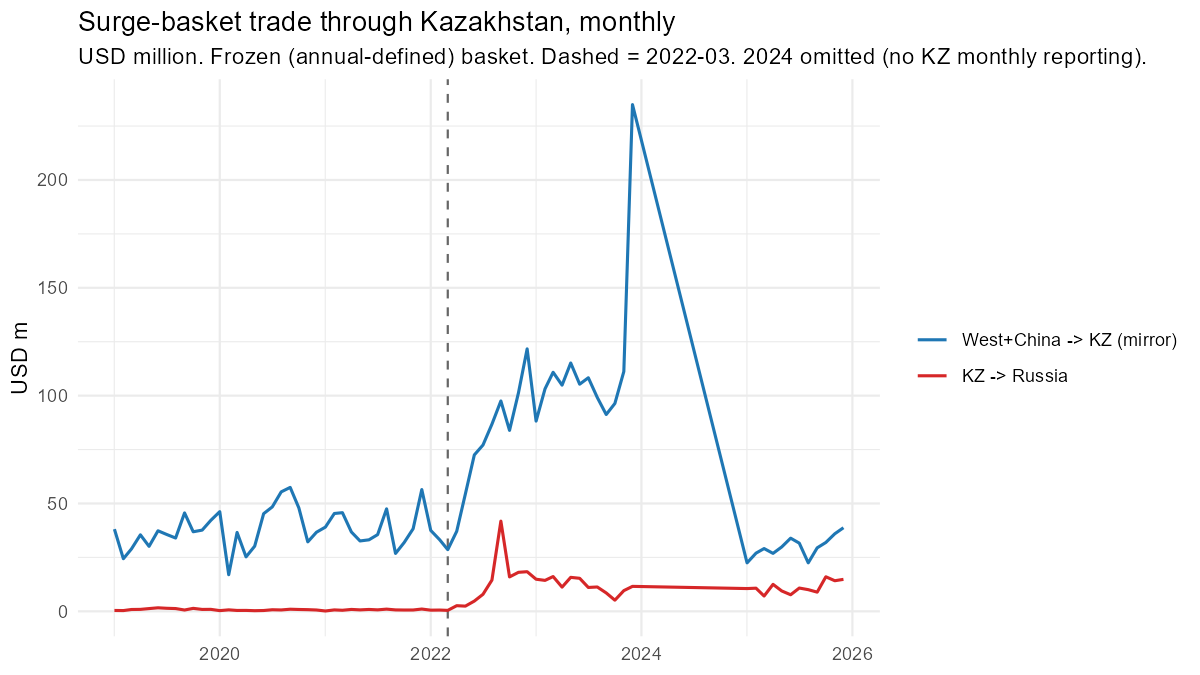
\includegraphics[width=.92\textwidth]{rq1_fig_monthly.png}
\caption{Торговля в рамках корзины всплеска через Казахстан, помесячно. Млн долл. США;
синий — зеркальный экспорт Запада и Китая в Казахстан, красный — экспорт Казахстана в
Россию. 2024 год опущен (месячная отчётность Казахстана в Comtrade приостановлена после
2024m2). Пунктирная линия: март 2022 года. Источник: UN Comtrade.}
\label{fig:monthly}
\end{figure}

\begin{figure}[t]
\centering
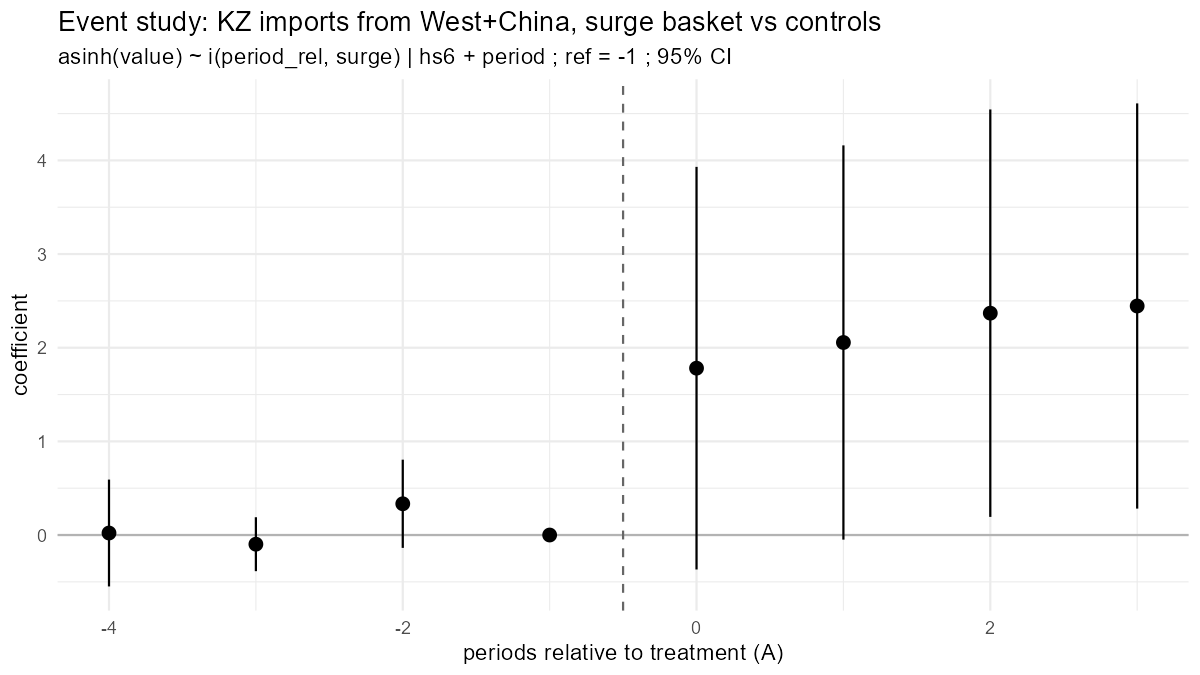
\includegraphics[width=.92\textwidth]{rq1_fig_eventstudy.png}
\caption{Анализ событий методом разности разностей, корзина всплеска против контрольных
позиций:
$\text{asinh}(y_{it}) = \sum_{k\neq -1}\beta_k\,(\text{всплеск}_i \times \mathbf{1}[t - 2022 = k])
+ \mu_i + \lambda_t + \varepsilon_{it}$, фиксированные эффекты HS6 и года, 95\%-е
доверительные интервалы кластеризованы по HS6, базовый год 2021. Источник: UN Comtrade.}
\label{fig:es}
\end{figure}

\subsection{Разность разностей}\label{sec:did}

\paragraph{Спецификация и идентифицирующие предпосылки.} На годовой панели мы оцениваем
$\text{asinh}(y_{it}) = \gamma\,(\text{treated}_i \times \text{post}_t) + \mu_i + \lambda_t +
\varepsilon_{it}$ с фиксированными эффектами HS6 и года и стандартными ошибками,
кластеризованными по HS6 (75 позиций, 8 лет; базовый год 2021). Нулевые значения часто
встречаются на исходящем плече до шока и редко — после (23\% ячеек корзины всплеска нулевые
в 2018--2021 годах против 3\% в 2022--2025 годах), поэтому мы приводим спецификацию asinh
наряду с оценкой Пуассона (PPML) в уровнях, которая обрабатывает нули без трансформации и
взвешивает по величине. Показатель $y$ измерен в исходных долларах США, поэтому при
существенной массе нулевых и близких к нулю значений в предпериоде коэффициент asinh не
имеет единой чистой интерпретации в процентном изменении по всем ячейкам; обе спецификации
согласуются по знаку и значимости, но не по подразумеваемой величине (точечная оценка asinh
соответствует эффекту уровня в несколько раз больше, чем $3.5\times$ по PPML), что является
одной из причин, по которой мы опираемся на знак и структурные переломы, а не на величину
коэффициента asinh (Таблица~\ref{tab:did}). Идентификация требует параллельных траекторий в
отсутствие шока (совместный тест трёх коэффициентов взаимодействия предпериода не отвергает
нулевую гипотезу: $p = 0.42$ по входящему потоку, $p = 0.78$ по исходящему) и отсутствия
опережающей реакции (полное исключение 2022 года либо перенос года «лечения» на 2023 год
меняет $\gamma$ лишь умеренно, до $2.71$; см. ниже). Гражданские контрольные позиции не
являются полностью «чистыми»: их экспорт в Россию также переламывается в 2022 году (см.
«Смешение с реформой» ниже), поэтому $\gamma$, если что, занижена относительно эффекта в
масштабах всей экономики. Корзина всплеска \emph{отбирается по результату пост-периода}, что
механически завышает $\gamma$; именно перестановочный тест, согласованный с правилом
отбора, приведённый ниже, а не кросс-секционная регрессия, отвечает на этот вопрос, а также
на вопрос о кросс-секционной зависимости, которую порождает единая общая дата «лечения». Мы
также приводим $p$-значения wild-cluster-бутстрапа (мало кластеров, внутригрупповая
серийная корреляция по HS6) и корректируем их по Холму для четырёх результатов по корзине
всплеска. И аналитические, и бутстраповские стандартные ошибки кластеризуются внутри HS6, но
рассматривают позиции как независимые; при единой общей дате «лечения» и шоке, который
одновременно затрагивает связанные товарные позиции, это оптимистичное допущение.
Приведённые ниже $p$-значения рандомизационного вывода не опираются на это допущение (они
пересэмплируют целые истории «лечения») и являются тем выводом, на который мы опираемся.

\paragraph{Результаты.} Таблица~\ref{tab:did} приводит $\gamma$ для корзины всплеска,
внешне составленного приоритетного списка и плацебо. По корзине всплеска экспорт в Россию
растёт на $\gamma = 2.44$ ($p = 0.013$; wild-бутстрап $p = 0.010$; скорректированный по
Холму $p = 0.039$; оценка Пуассона в уровнях $3.5\times$, $p = 0.02$). Входящий поток
(Запад + Китай) растёт на $\gamma = 2.10$ ($p = 0.05$, незначим после коррекции Холма);
только западная компонента — на $1.73$ ($p = 0.08$); собственная заявленная импортная
статистика Казахстана — на $1.88$ ($p = 0.004$, Холм $p = 0.016$). Внешне составленный
приоритетный список, не отобранный по казахстанскому результату, даёт тот же паттерн
($\gamma = 2.88$ по исходящему потоку, $2.12$ по входящему). Эффект по исходящему потоку
выдерживает две дополнительные проверки: добавление фиксированных эффектов
«дециль размера$\times$год» (размер входящего потока до 2022 года) даёт
$\gamma = 2.29$ ($p = 0.003$), а исключение 2022 года повышает её до $2.71$ ($p = 0.012$).
Те же контроли «размер$\times$год» снижают коэффициент входящего потока «Запад + Китай» до
$1.28$ ($p = 0.05$), что согласуется с тем, что входящее плечо на протяжении всего анализа
слабее исходящего. Ужесточение порога отбора с удвоения до $2.5\times$ или $3\times$
повышает исходящую $\gamma$ примерно до $3.1$. Смягчение порога до $1.5\times$ (40 позиций)
снижает её до $1.6$ ($p = 0.08$). Джекнайф с последовательным исключением одной группы HS2
показывает, что эффект несёт группа HS~85: её исключение (13 из 29 позиций) даёт
$\gamma = 1.36$ ($p = 0.21$); остальные шесть групп, исключаемые по одной, дают
$\gamma = 2.51$ (исключена HS~39), $2.48$ (HS~40), $2.67$ (HS~61), $2.28$ ($p = 0.06$;
HS~84), $3.16$ (HS~90) и $2.59$ (HS~96) — все значимы на уровне 5\%, кроме HS~84 на уровне
6\%. Таким образом, точечная оценка существенно зависит от позиций электротехнического
машиностроения, где и сконцентрирована переориентация; знак и значимость на уровне ниже 5\%
от этого не зависят, за исключением случая исключения крупнейшей товарной группы.

Три оговорки не позволяют нам опираться на идентификацию исключительно на этой
кросс-секционной регрессии (полная батарея приведена в Приложении~\ref{app:did}). Во-первых,
перестановочный тест, согласованный с правилом отбора: когда мы навязываем нулевую гипотезу
путём перестановки годовых меток внутри каждой позиции HS6 и повторного применения правила
удвоения, правило в среднем отбирает пять позиций (никогда не 29, как в наблюдаемых данных,
поэтому само \emph{существование} корзины всплеска не является случайным артефактом,
$p < 0.001$); версия, сохраняющая тренд и лишь сдвигающая перелом за пределы календарного
2022 года, сохраняя автокорреляцию и трендовый уровень каждой позиции, даёт тот же результат
(нулевое среднее — пять позиций, $p < 0.001$), поэтому именно привязка к 2022 году, а не
уже существовавший тренд, улавливается правилом отбора. Однако наблюдаемое значение
$\gamma = 2.44$ надёжно попадает внутрь нулевого распределения самого коэффициента,
согласованного с правилом отбора (среднее нулевого распределения $2.79$, ст. откл. $1.50$;
$p = 0.58$ для $|\gamma^{\text{perm}}| \ge |\gamma^{\text{obs}}|$), поэтому \emph{величина}
коэффициента не отделима от отбора, и мы не рассматриваем её как идентифицированный размер
эффекта. Во-вторых, два порога отбора работают по-разному: 55 из 75 кандидатных позиций
проходят удвоение по исходящему потоку, но лишь 41 — по входящему, поэтому требование
выполнения обоих условий является реальным фильтром именно по импортной стороне, а не
только по оттоку в Россию; это частичная проверка против отбора корзины исключительно по
исходящему результату, который затем использует разность разностей. В-третьих, строка
плацебо: присвоение фиктивного «лечения» крупнейшим гражданским позициям даёт
$\gamma = -0.95$ ($p = 0.001$; крупные потребительские товарные позиции сократились после
2022 года, как и предсказывала бы девальвация тенге), что показывает неоднородность
контрольной группы по тренду. Устойчивость коэффициента по корзине всплеска к контролям
«дециль размера$\times$год» частично снимает эту проблему, и мы не рассматриваем плацебо как
подтверждение. В совокупности кросс-секционная разность разностей документирует исходящую
переориентацию, но не идентифицирует её самостоятельно; основную нагрузку несут структурные
переломы (раздел~\ref{sec:shock}) и приведённое ниже сопоставление с соседними странами.
Показатель «зеркального разрыва» (входящий поток по данным партнёров минус заявленный
казахстанский импорт) не изменяется ($\gamma = 0.54$, $p = 0.81$).

\begin{table}[t]
\centering
\caption{Разность разностей: $\gamma$ при $\text{лечение}\times\text{после}$ в
$\text{asinh}(y_{it}) = \gamma(\text{лечение}_i\times\text{после}_t) + \mu_i + \lambda_t +
\varepsilon_{it}$, фиксированные эффекты HS6 и года, устойчивые к кластеризации стандартные
ошибки (по HS6) в скобках. Строки «корзина всплеска» и «приоритетный список» имеют
$N = 600$ (75 позиций $\times$ 8 лет); строка плацебо имеет $N = 200$ (25 гражданских
позиций). Строка «остаточный список» оценена на очищенной выборке, $N = 368$ (26 остаточных
позиций плюс 20 гражданских контрольных позиций, из которых исключена сама корзина
всплеска; обзор JIE, раунд 2, рецензент B, замечание N1 — в более ранней версии этой строки
в качестве «контроля» использовалась полная панель, что приводило к двойному учёту 29
позиций корзины всплеска; здесь это исправлено). Корзина всплеска отобрана по входящему
(Запад + Китай) и исходящему потокам; приоритетный список (50 кодов) составлен извне.
Строка 1 (корзина всплеска) и строка 2 (приоритетный список) оценены на полной панели из
75 позиций; строка 3 (остаточный список) оценена на очищенной выборке из 46 позиций,
описанной выше, поэтому её контрольная группа отличается от строк 1--2. В строке 1 звёздочки
не приводятся: величина коэффициента по корзине всплеска не отделима от отбора выборки
(Панель C), включая столбец заявленного казахстанского импорта, чью видимую значимость
следует оценивать по нулевому распределению рандомизационного вывода Панели C для этой
корзины, а не воспринимать буквально. Звёздочка в строке «остаточный список» отражает
$p$-значение wild-cluster-бутстрапа — надёжную статистику при 46 кластерах.}
\label{tab:did}
\footnotesize
\setlength{\tabcolsep}{5pt}
\begin{tabular}{@{}lcccc@{}}
\toprule
& Экспорт в & Входящий & Входящий & Заявленный \\
Отобранная группа & Россию & (Запад+Китай) & (Запад) & импорт КЗ \\
\midrule
\multicolumn{5}{@{}l}{\emph{Панель A. asinh DiD, $\gamma$ (устойчивые к кластеризации ст. ошибки по HS6)}} \\
Корзина всплеска (29 HS6)                 & 2.44 (0.96) & 2.10 (1.06) & 1.73 (0.98) & 1.88 (0.63) \\
Приоритетный список, внешний (50 HS6) & 2.88 (0.74)$^{***}$ & 2.12 (0.71)$^{**}$ & 1.93 (0.67)$^{**}$ & 2.94 (0.53)$^{***}$ \\
\quad\emph{из них 26 позиций, очищенный гражданский контроль} & 1.94 (0.90)$^{\dagger}$ & 1.12 (0.83) & --- & --- \\
Плацебо (крупнейшие гражданские позиции)      & --- & $-0.95$ (0.25)$^{**}$ & --- & --- \\
\midrule
\multicolumn{5}{@{}l}{\emph{Панель B. Пуассон (PPML) DiD в уровнях, $e^{\beta}$ (мультипликативно)}} \\
Корзина всплеска (29 HS6)                 & $3.5\times^{*}$ & $2.4\times^{***}$ & --- & --- \\
\midrule
\multicolumn{5}{@{}l}{\emph{Панель C. Рандомизационный вывод, согласованный с правилом отбора, и случайная корзина, экспорт в Россию}} \\
\multicolumn{5}{@{}l}{\quad корзина всплеска, нулевое распределение по правилу: среднее $2.79$, ст. откл.\ $1.50$; $P(|\gamma^{\text{perm}}|\ge 2.44) = 0.58$} \\
\multicolumn{5}{@{}l}{\quad корзина всплеска, нулевое распределение существования: $P(\text{правило отбирает}\ge 29\text{ позиций}\mid H_0) = 0.000$} \\
\multicolumn{5}{@{}l}{\quad приоритетный список, нулевое распределение случайной корзины из 50 позиций: среднее $0.00$, ст. откл.\ $0.97$; $P(|\gamma^{\text{perm}}|\ge 2.88) = 0.002$} \\
\bottomrule
\end{tabular}

\vspace{2pt}
\footnotesize $^{*}$ $p<0.05$, $^{**}$ $p<0.01$, $^{***}$ $p<0.001$ (устойчивые к
кластеризации; до поправки на множественное тестирование); $^{\dagger}$ $p<0.05$ по
wild-cluster-бутстрапу — надёжная статистика при 46 кластерах (аналитическое $p$, устойчивое
к кластеризации, ненадёжно при таком числе кластеров). После поправки Холма по четырём
результатам корзины всплеска экспорт в Россию и заявленный импорт КЗ остаются значимыми на
уровне 5\%. Строки «корзина всплеска» и «приоритетный список» в Панели A имеют $N = 600$
(75 позиций $\times$ 8 лет); строка «остаточный список» имеет $N = 368$ (46 позиций
$\times$ 8 лет, очищено от корзины всплеска и по группе «лечения», и по контрольной
группе); строка плацебо имеет $N = 200$. $p$-значение wild-cluster-бутстрапа для строки
«остаточный список» — $0.035$ по исходящему потоку, $0.238$ по входящему. Панель B: точные
коэффициенты PPML $\beta = 1.26$ ($p = 0.02$) по исходящему потоку и $\beta = 0.85$
($p < 10^{-4}$) по входящему. Панель C: \emph{величина} коэффициента по корзине всплеска не
отделима от отбора по постпериодному результату, но само \emph{существование} корзины из 29
позиций не является случайным артефактом ни при свободной, ни при сохраняющей тренд
перестановке; коэффициент приоритетного списка, напротив, необычен относительно случайной
корзины из 50 любых позиций HS6, что согласуется с тем, что он несётся существенно, хотя и
не полностью, действительно затронутыми лечением позициями корзины всплеска, которые он
содержит: собственная, меньшая по величине разность разностей 26 остаточных позиций,
оценённая на очищенном контроле, независимо значима по исходящему потоку (строка 3).
\end{table}

\paragraph{Смешение с реформой.} Три обстоятельства отделяют переориентацию от
ориентированной вовне политической повестки 2022 года. Во-первых, гражданская контрольная
корзина ведёт себя так, как не может объяснить широкая реформа: по годовым данным её
входящий поток вовсе не движется в 2022 году, а хотя экспорт в Россию по ней и сдвигается
(общий эффект торговли с Россией), этот сдвиг намного меньше, чем у корзины всплеска по тому
же тесту, а месячный перелом исходящего потока корзины всплеска ещё более резкий. Во-вторых,
исходящий перелом датирован 2022m5 — до июньского референдума и ноябрьских выборов.
В-третьих, и наиболее прямо: экспорт Армении по корзине всплеска в Россию вырос с
\$7--15 млн в год до \$71 млн в 2022 году и \$93 млн в 2023 году, а Кыргызской Республики —
с \$1--7 млн до \$12 млн и \$30 млн, в те же сроки, причём ни в одной из этих стран не
проводилось реформы «Новый Казахстан». Направление также верное: товары поступают от
западных стран-респондентов и движутся далее в Россию, а не наоборот.

\section{Что удерживает Казахстан}\label{sec:capture}

\subsection{Удерживаемая торговая маржа}

Мы измеряем, что удерживает Казахстан, на \emph{приростном} потоке (экспорт в Россию сверх
базового уровня до 2022 года, около \$479 млн кумулятивно за 2022--2025 годы), поскольку
именно эту часть и породила переориентация. Прирост в \$479 млн измерен относительно
неизменного контрфактического уровня — среднего за 2018--2021 годы (\$11 млн в год);
поскольку сам исходящий ряд до 2022 года снижался (\$17 млн$\to$\$8 млн), это консервативный
выбор: экстраполяция предшествующего тренда привела бы контрфактический уровень почти к
нулю к 2024 году и повысила бы прирост примерно до \$521 млн, расширив каждую последующую
цифру примерно на десятую часть. При сопоставлении с приростным \emph{западным} входящим
потоком в около \$887 млн сквозной проход составляет примерно половину; при сопоставлении с
приростным входящим потоком «Запад + Китай» в около \$3.2 млрд — одну шестую.\footnote{В
этом разделе фигурируют три показателя сквозного прохода, на разных выборках и базах:
\emph{приростное} отношение к западному входящему потоку ($\approx 0.54$, по агрегату
2022--2025 годов за вычетом базового уровня) и к «Запад + Китай» ($\approx 0.15$, «одна
шестая»); последнее вычислено только на 2022--2024 годах, поскольку показатель «Запад +
Китай» за 2025 год в Таблице~\ref{tab:magnitudes} отражает только Запад (Китай ещё не
отчитался), и включение его в прирост «Запад + Китай» занизило бы его по построению;
показатель на смешанной базе 2022--2025 годов даёт то же отношение с точностью до двух
знаков после запятой. \emph{Агрегированное отношение по сопоставленным ячейкам}
($\approx 0.11$, сумма стоимости реэкспорта к сумме стоимости входящего потока по 112
сопоставленным ячейкам HS6$\times$период), используемое ниже в обсуждении весового
отношения, — третья, отдельная конструкция.} Входящее плечо идентифицировано слабее из
двух (его коэффициент DiD теряет значимость при контролях «размер$\times$год» и после
поправки на множественное тестирование, раздел~\ref{sec:did}), поэтому показатель сквозного
прохода следует воспринимать как ориентировочный, а не точный. Оставшиеся
\$887 млн${}-{}$\$479 млн${}={}$\$408 млн западного прироста раскладываются лишь примерно на
\$41 млн экспорта далее в страны, отличные от России (экспорт Казахстана по корзине
всплеска в остальной мир почти не движется), и примерно \$367 млн внутреннего поглощения,
запасов и разрыва между c.i.f. и зеркальным измерением, так что разрыв сквозного прохода не
скрывает реэкспорт через третьи страны. Западная база здесь релевантна для переориентации, и
мы используем именно её.

Свидетельства об удельной стоимости согласуются с картиной коридора и сами по себе не
идентифицируют удерживаемую маржу. На базе c.i.f./f.o.b. (цена f.o.b. реэкспорта Казахстана
против зафиксированной цены c.i.f. при импорте, которая включает фрахт для страны, не
имеющей выхода к морю) медианное отношение по сопоставленным ячейкам HS6$\times$период
составляет \textbf{0.73} (годовые данные, $n = 112$; $0.70$ по месячным). На базе,
сопоставимой напрямую по f.o.b., против цены, заявленной экспортёром на границе партнёра,
медиана составляет \textbf{1.6} (годовые данные; $1.5$ по месячным), разница примерно
соответствует фрахту на входящем плече. Ни одно из отношений не является выделяющимся
(гражданская контрольная корзина даёт $0.59$ и $0.94$ по двум базам), а регрессия
сквозного прохода цены слаба по обеим (наклоны $0.20$ и $0.48$, значимы лишь в годовой
спецификации по f.o.b.).

Два признака говорят против внутренней трансформации, хотя ни один не является решающим.
Первый — весовое отношение (реэкспортированный тоннаж к импортированному тоннажу в
сопоставленной ячейке), которое составляет $0.08$ по медиане и $0.11$ в агрегате, близко к
агрегированному сквозному проходу стоимости по сопоставленным ячейкам (медиана $0.15$,
агрегат $0.11$). Агрегированное весовое отношение и агрегированный сквозной проход стоимости
— одна и та же конструкция в разных единицах, и здесь они совпадают на уровне $0.11$,
поэтому весовое отношение ниже единицы — в значительной степени факт сквозного прохода,
учитывая, что лишь часть импортированного тоннажа вообще реэкспортируется в Россию, а не
свидетельство о наборе веса на единицу транзитного товара. Одиннадцать процентов ячеек всё
же имеют весовое отношение выше $1.05$, при широком межквартильном размахе (от $0.02$ до
$0.49$); согласно интерпретации сквозного прохода, этот верхний хвост отражает скорее
временны́е сдвиги и запасы, чем переработку. Если ограничиться шестью ячейками
HS6$\times$период, близкими к чистому транзиту, где сквозной проход стоимости близок к
единице, медианное весовое отношение составляет $0.74$ ($0.26$ и $0.94$ по квартилям, на
$n = 6$), не показывая признаков добавления местных ресурсов к товарам, которые
действительно проходят транзитом, хотя и на тонком срезе корзины. Выгрузка данных Comtrade
в том виде, как она получена, содержит стоимость и чистый вес, но не физическое количество,
поэтому более чистый тест на трансформацию на единицу продукции здесь недоступен.

Второй признак — разброс в наценке f.o.b., который не является сигналом переработки. Наценка
неравномерна по уровням списка,\footnote{Приоритетный список опубликован с товарами,
сгруппированными по уровням (Уровни~1--2 — наиболее чувствительные, Уровни~3--4 —
последовательно менее чувствительные); мы сохраняем опубликованные обозначения уровней без
изменений и используем их лишь для описания того, где в списке возникают высокие наценки.
Уровень~1 = HS 8542 (интегральные схемы); Уровень~2 добавляет трансиверы, конденсаторы,
разъёмы; Уровни~3--4 — более широкий круг машин, приборов и компонентов.} с медианами по
уровням около четырёх для Уровней~2 и~4A, но около единицы для Уровней 3B и 4B и лишь
$0.47$ для Уровня~1; высокие кратные значения приходятся примерно на половину сопоставленного
валового потока (Рисунок~\ref{fig:wedge}). Неравномерная наценка, сконцентрированная в
подмножестве позиций, — это паттерн наценки за дефицит на товары, которые стало труднее
приобрести напрямую, а не равномерная, сквозная наценка, которую давала бы маржа
переработки. Это тот же паттерн, который \citet{feenstrahanson2004entrepot} документируют
для антрепотной торговли Гонконга китайскими товарами, где реэкспортная наценка наибольшая
там, где посредник добавляет стоимость подбора и дефицита, а не физической трансформации;
наценка здесь если и отличается, то в меньшую и более шумную сторону. Взвешенная по
стоимости агрегированная наценка ниже единицы, определяется небольшим числом ячеек с
крупным входящим потоком и заниженным декларированием исходящей стоимости
\citep{fisman2004missing}. Наценка не фиксирует удерживаемую маржу, которую мы берём далее
из национальных счетов.

\begin{figure}[t]
\centering
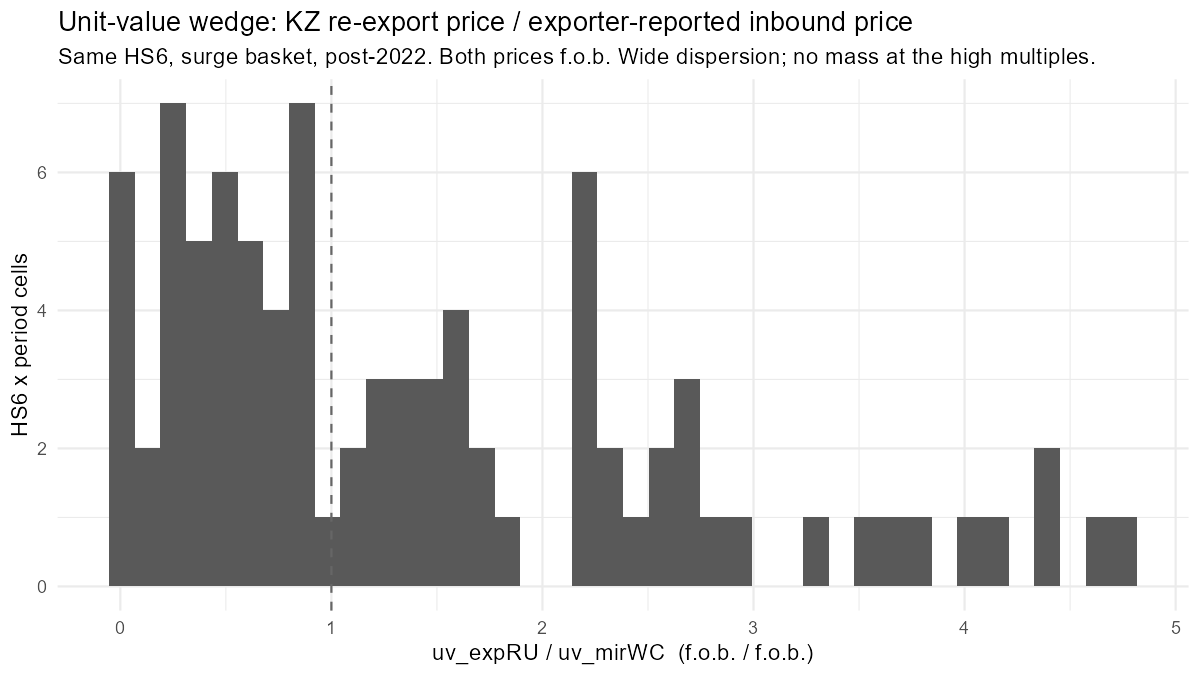
\includegraphics[width=.72\textwidth]{rq2a_fig_wedge_hist.png}
\caption{Наценка по удельной стоимости: цена реэкспорта Казахстана к заявленной
экспортёром входящей цене (на базе f.o.b.), те же позиции HS6, корзина всплеска, после 2022
года. Широкий разброс, с высокими кратными значениями в подмножестве позиций (медианы по
уровням около четырёх для Уровней~2 и~4A, около единицы в остальных): паттерн, который даёт
наценка за дефицит, а не равномерная, сквозная наценка переработки.}
\label{fig:wedge}
\end{figure}

\subsection{Распространение через таблицу «затраты--выпуск»}

Пусть $m$ — оптово-транспортная маржа, которую Казахстан удерживает на транзитном товаре как
долю его стоимости, $\bar v^{TT}$ — средний мультипликатор внутренней добавленной стоимости
для его секторов торговли, транспорта и складского хранения, а $\bar v^{M}$ — тот же
показатель для обрабатывающей промышленности. Внутренняя добавленная стоимость на доллар
валового переориентированного потока равна $m\,\bar v^{TT}$; на доллар внутреннего
промышленного производства она равна $\bar v^{M}$
\citep{koopman2014tracing,johnson2012accounting}. По блоку Казахстана OECD ICIO
$\bar v^{TT} = 0.79$ и $\bar v^{M} = 0.76$ — значения достаточно близки, так что шаг
распространения почти не влияет на результат: итог по существу определяется одним лишь $m$
относительно полной внутренней стоимости $\bar v^{M}$.

Мы принимаем $m$ как то, что удерживает торговый посредник, покупающий товар оптом и
перепродающий его без розничного звена и без физической трансформации: наценка фрахта и
страхования между c.i.f. и f.o.b. плюс оптовая (не розничная) торговая маржа. Таблица
ресурсов Бюро национальной статистики Казахстана \citep{qazstat2023io} задаёт границы: доля
\emph{транспортной} маржи для машин и электроники составляет около 1\% стоимости в базовых
ценах, а \emph{полная} торгово-транспортная маржа (которая также несёт розничное звено,
которое коридор никогда не выполняет) — около 49\%. Оптово-транспортная маржа находится в
нижней части этого диапазона. Наценка фрахта и страхования между ценами f.o.b. и c.i.f.
обычно составляет несколько процентов (коэффициент c.i.f./f.o.b., применяемый в торговой
статистике, — около 1.06); зафиксированные маржи c.i.f./f.o.b. для постсоветских экономик
слишком зашумлены, чтобы использовать их напрямую, а для нескольких из них зафиксированный
показатель f.o.b. превышает показатель c.i.f. \citep{arvis2010landlocked}, поэтому мы на них
не опираемся. Добавление оптовой распределительной маржи в несколько пунктов к
однозначной наценке фрахта даёт нижнюю часть диапазона Бюро национальной статистики.
Компонента торговой маржи в таблице ресурсов сама по себе (без транспорта) составляет 48\%
для машин и электроники — почти весь потолок в 49\%, что подтверждает, что транспорт —
малая часть полной маржи для этой категории, но само по себе не фиксирует чисто оптовую
долю: таблица не разделяет опт и розницу, поэтому не может самостоятельно подтвердить
диапазон, призванный исключить розничное звено. Мы используем диапазон \textbf{6--14\%} и
трактуем его как калибровку, а не оценку, поскольку ни построчная маржа, ни разделение
опт/розница в наших данных не идентифицированы. Поскольку $\bar v^{TT} \approx \bar v^{M}$,
шаг «затраты--выпуск» не выполняет никакой работы, поэтому итог напрямую зависит от $m$, и
мы приводим его как диапазон. (Мы также не используем сопоставленную по ячейкам наценку по
удельной стоимости для фиксации $m$: цензурирование ячеек с отрицательной маржой завышает
валовую маржу примерно до 34\%, тогда как взвешенный по стоимости агрегат отрицателен, и оба
эти показателя являются артефактами несовпадения базы c.i.f./f.o.b. и занижения
декларируемой исходящей стоимости, а не мерой удерживаемой внутренней стоимости. Мы не
можем полностью согласовать показатель 34\% с нашим диапазоном: граница занижения
отчётности, которую мы можем обосновать в других частях данных (13--21\%, ниже), сама по
себе недостаточно велика, чтобы объяснить этот разрыв, поэтому часть разрыва в 34\%,
вероятно, отражает несовпадение базы, а не только занижение декларирования, но мы не можем
разделить эти два эффекта на имеющихся данных и рассматриваем 34\% как верхнюю границу,
которую должен выдержать качественный вывод работы, а не как подтверждённую точечную
оценку.) Внутренняя добавленная стоимость на переориентированный доллар тогда составляет
$m\,\bar v^{TT} \approx$ \textbf{5--11\%}, медианно около \textbf{8\%}, против
\textbf{76\%} на доллар внутреннего промышленного производства, так что переориентированный
доллар создаёт примерно на порядок меньше внутренней стоимости, чем произведённый. Из
\$479 млн приростного экспорта в Россию после 2022 года Казахстан удерживает в качестве
внутренней добавленной стоимости примерно \textbf{\$23--53 млн}.

Поскольку шаг распространения близок к тождественному, итоговый показатель является прямой
функцией $m$, и читатель может подставить иную маржу напрямую (Приложение~\ref{app:io},
Таблица~\ref{tab:appd}, приводит полную развёртку, перекрёстную проверку по таблице
«затраты--выпуск» и детализацию наценки по сопоставленным ячейкам). Развёртывая $m$ по всему
диапазону Бюро национальной статистики: на транспортном конце ($m \approx 1\%$)
переориентированный доллар захватывает примерно одну сотую произведённого; в нашем
диапазоне 6--14\% — от одной шестнадцатой до одной седьмой; интерпретация «коридор, а не
завод» (переориентированный доллар стоит порядка одной десятой произведённого) сохраняется
при любом $m$ вплоть до примерно $12\%$. Она ослабевает до «около одной пятой» лишь при
$m \approx 19\%$, до «около трети» при $m \approx 32\%$ и достигает примерно половины лишь
при $m \approx 49\%$ — полной торгово-транспортной марже, включающей розничное звено,
которое коридор никогда не выполняет. Цензурированная валовая маржа по сопоставленным
ячейкам ($34\%$), даже принятая буквально, всё равно оставляет переориентированный доллар на
уровне примерно трети произведённого. Таким образом, качественный вывод устойчив к любой
марже, которую может обосновать оптово-транспортная интерпретация; он не выполняется лишь в
том случае, если коридор фактически захватывает почти полную наценку, включающую розницу.
Единственное свидетельство, которое напрямую говорит о столь крупной наценке, —
взвешенная по стоимости агрегированная наценка по удельной стоимости, которая сама по себе
ниже единицы; мы трактуем это лишь как наводящее свидетельство, поскольку оно занижено
из-за занижения декларирования исходящей стоимости и несовпадения базы c.i.f./f.o.b.

Мультипликаторы имеют сравнительно малое значение. Даже при $\bar v^{M} = 0.40$ отношение
составляет примерно один к пяти; пересчёт $\bar v^{TT}$ и $\bar v^{M}$ по симметричной
таблице «затраты--выпуск» Бюро национальной статистики (68 продуктов, 2023 год) вместо
OECD ICIO даёт $\bar v^{TT} = 0.89$ и $\bar v^{M} = 0.74$, смещая отношение
переориентированного к произведённому с примерно одной десятой к одной восьмой — всё ещё
порядок величины. Занижение декларирования сдвигает результат лишь до определённого предела:
чтобы внутренняя добавленная стоимость достигла одной пятой \emph{от валового
переориентированного потока} (более требовательный ориентир, чем одна пятая произведённого
доллара, которую уже достигает $m \approx 19\%$), торговая маржа должна была бы составить
около $25\%$, что, при неизменной зафиксированной стоимости импорта, требует занижения
декларируемого экспорта в Россию на $13$--$21\%$. Занижение отчётности такого масштаба
находится в диапазоне, обнаруженном для транзитной торговли \citep{fisman2004missing}, и не
может быть исключено; но даже при этой границе Казахстан удерживает не более примерно
четверти того, что захватывает производящая экономика.

\subsection{Фискальные и макроэкономические эффекты}

Обусловленный переориентацией поток (приростный экспорт в Россию сверх базового уровня до
2022 года) составляет около \$479 млн кумулятивно за 2022--2025 годы (\$107--134 млн в год).
Таможенная пошлина на него, при общем внешнем тарифе ЕАЭС в 4--8\% на долю, формально
оформляемую в Казахстане, составляет порядка \textbf{\$22 млн за четыре года} (около
\$5 млн в год); чистый НДС на импорт близок к нулю, поскольку последующая поставка в Россию
является внутрисоюзной и облагается по нулевой ставке. Годовые таможенные доходы Казахстана
составляют порядка \$4--5 млрд, поэтому переориентация добавляет существенно менее 1\%. На
макроуровне валовой переориентированный поток, около \$0.6 млрд в год с учётом входящего и
исходящего плеч вместе, составляет 0.2--0.3\% ВВП; профицит текущего счёта 2022 года,
накопление резервов в 2023--2025 годах и рост добавленной стоимости в сфере услуг на порядок
величины слишком велики, чтобы объясняться этим потоком.

\section{(Не)инвестиционный отклик}\label{sec:investment}

Если бы шок спроса порождал внутреннюю добавленную стоимость, следовало бы ожидать роста
инвестиций в секторах, через которые проходит поток. Мы такого роста не находим, хотя при
всего четырёх пост-2022-х годах тест на число сделок позволяет исключить лишь крупный
отклик, а не умеренный.

Заключение сделок в обрабатывающей промышленности торгуемых товаров, транспорте и логистике
и в оптовой дистрибуции происходит с интенсивностью \textbf{7.6 в год} в 2015--2021 годах и
\textbf{7.2 в год} в 2022--2025 годах (отношение интенсивностей по Пуассону — 0.96, 95\%-й
доверительный интервал 0.59--1.53). Два самых «тонких» года — 2015-й, с единственной
зафиксированной сделкой на этапе, когда базы данных ещё наращивали охват Казахстана, и
2022-й, год беспорядков (Рисунок~\ref{fig:mismatch}). Если исключить «тонкий» первый 2015
год, интенсивность до 2022 года составляет 8.7 в год, так что пост-период представляет собой
небольшое снижение по любой из баз. Если исключить провальный 2022 год, интенсивность в
2023--2025 годах составляет 8.7 в год (отношение интенсивностей 1.14, 95\%-й доверительный
интервал 0.69--1.86). Тест обладает мощностью 80\% лишь против роста примерно на 80\% или
более, поэтому он исключает всплеск заключения сделок, но не умеренный сдвиг. Больше о
происходящем говорит структура этой активности. Заявленная \emph{стоимость} сделок в этих
секторах растёт, но концентрируется в передаче собственности на существующие или проблемные
активы, а не в новых производственных мощностях: национализация ArcelorMittal Temirtau в
Qarmet (2023), Eurocopter Kazakhstan и локомотиворемонтный завод (повторные национализации,
2024) и консолидация железнодорожно-грузовых и экспедиторских активов на \$0.8 млрд в 2025
году. Гринфилд-сделки и сделки по созданию новых мощностей в среднем составляют менее двух в
год и никогда не превышают четырёх, без роста после 2022 года. За весь период 2015--2025
годов данные не содержат \textbf{ни одной} сделки в конкретных товарных позициях, которые
доминируют в переориентации, хотя мы не придаём этому большого значения, поскольку базовый
уровень сделок в этих узких позициях был близок к нулю и до 2022 года, так что нулевой
показатель пост-периода сам по себе несёт мало информации. Мы засчитали бы как
положительный инвестиционный отклик любую гринфилд-сделку или сделку по расширению мощностей
в любой из трёх баз данных, отнесённую к позиции HS6 корзины всплеска \emph{либо} к её
родительскому классу электротехнического машиностроения, компонентов или приборостроения.
По этому правилу число сделок равно нулю как до, так и после, и информативной статистикой
является приведённый выше отраслевой тест интенсивности, который исключает сдвиг порядка
удвоения или более.

\begin{figure}[t]
\centering
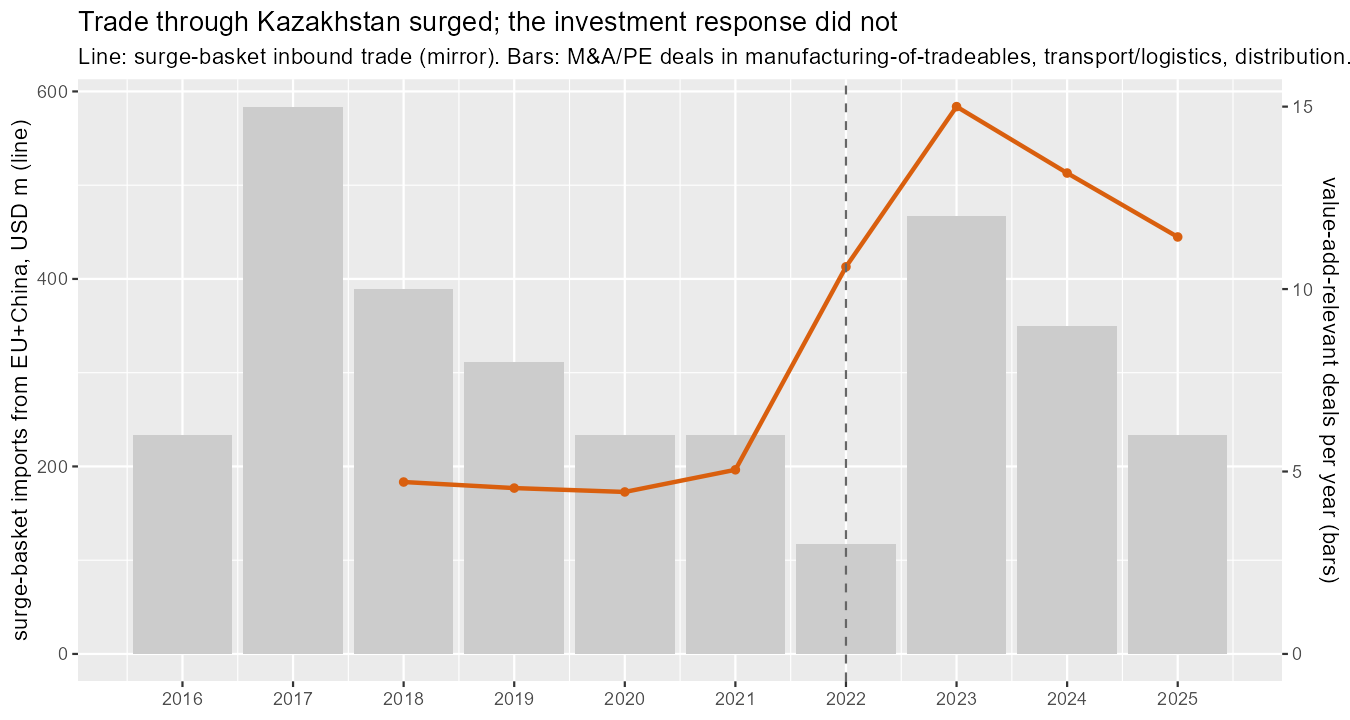
\includegraphics[width=\textwidth]{valueadd_fig_mismatch.png}
\caption{Торговля через Казахстан резко выросла; инвестиционный отклик — нет. Линия:
\emph{западный} входящий поток корзины всплеска (зеркальный показатель по данным партнёров),
млн долл. США (левая ось; итог «Запад + Китай» в несколько раз больше, но уже рос до 2022
года). Столбцы: годовое число сделок M\&A/PE в обрабатывающей промышленности торгуемых
товаров, транспорте и логистике и оптовой дистрибуции (правая ось). Пунктирная линия: 2022
год. Столбцы показаны с 2016 года; 2015 год с единственной зафиксированной сделкой опущен
(раздел~\ref{sec:investment}). Источник: UN Comtrade; Capital~IQ/PitchBook/Preqin.}
\label{fig:mismatch}
\end{figure}

Результат сохраняется по всем трём базам данных. Таблица~\ref{tab:dealsource} приводит
число сделок для одной и той же казахстанской выборки по каждому источнику; охват
различается по уровню (ориентированная на транзакции выборка Capital~IQ фиксирует больше
сделок среднего рынка M\&A, ориентированная на венчур PitchBook — больше небольших раундов
ранней стадии, Preqin — меньше и тех, и других), но ни один источник не показывает более
чем неизменную интенсивность заключения сделок в обрабатывающей промышленности или
логистике (5.1 к 5.2, 2.0 к 1.5 и 0.4 к 0.5 в год). В выборке Capital~IQ, которая лучше
всего отражает сделки среднего рынка в промышленности, которые и порождал бы настоящий
отклик в форме создания мощностей, число сделок в обрабатывающей промышленности,
транспорте и дистрибуции по существу не меняется до и после 2022 года (5.1 против 5.2 в
год).

\begin{table}[t]
\centering
\caption{Число сделок для казахстанской выборки, по источнику и периоду. Интенсивности — в
год за 7-летнее предпериодное окно (2015--21) и 4-летнее постпериодное окно (2022--25).
Консолидированная выборка без дублей — $N = 493$ сделки; подвыборка «обраб.
пром. + транспорт + дистрибуция» — $N = 82$ (53 до, 29 после).}
\label{tab:dealsource}
\footnotesize
\begin{tabular}{lrrr}
\toprule
Сделок в год (если не указано иное) & Cap.~IQ & PitchBk & Preqin \\
\midrule
Все сделки, 2015--21              & 24.0 & 14.6 & 3.7 \\
Все сделки, 2022--25              & 23.2 & 24.2 & 1.8 \\
Обраб. пром. + трансп. + дистриб., 2015--21 & 5.1 & 2.0 & 0.4 \\
Обраб. пром. + трансп. + дистриб., 2022--25 & 5.2 & 1.5 & 0.5 \\
Позиции корзины всплеска, 2015--25 (всего) & 0$^{a}$ & 0 & 0 \\
\bottomrule
\end{tabular}

\vspace{2pt}
\footnotesize $^{a}$ Две записи Capital~IQ помечены отраслевым тегом «электроника»
(производитель стального каната и финансовый холдинг) и являются ошибками классификации;
сделок в товарных позициях переориентации нет.
\end{table}

Казахстан наращивает мощности по сборке автомобилей (китайские марки, KIA, \v{S}koda) и
некоторые мощности по производству бытовой техники, но это предшествует переориентации и
во многом от неё не зависит, представляет собой крупноузловую сборку с низкой внутренней
добавленной стоимостью и обслуживает внутренний и евразийский потребительский рынок, а не
поток реэкспорта в Россию. Раскрытый пост-2022-й конвейер государственной инвестиционной
корпорации — это внутренние продовольствие, энергетика и инфраструктура, а не переработка в
рамках коридора \citep{qicaifcifc2026pe}. Единственный инвестиционный сигнал, связанный с
переориентацией, — консолидация трансграничных железнодорожно-грузовых и экспедиторских
активов в 2025 году, — углубляет роль Казахстана как экспедиторской операции, а не
производящей.

\section{Какой шлюз связывает?}\label{sec:why}

Порог в уравнении~\eqref{eq:build} задан на сумме, а не на произведении, поэтому ни одно
отдельное слагаемое уравнения~\eqref{eq:gates} не является определяющим само по себе; ниже
для Казахстана изложено то, что устанавливает каждый аргумент в
разделах~\ref{sec:shock}--\ref{sec:why} на своих собственных основаниях. Шлюз доступа к
рынку открыт: в рамках Евразийского экономического союза товар движется в Россию без
трансформации и без границы, поэтому $V_T$ велико. Два свидетельства являются наводящими, но
не доказательными (раздел~\ref{sec:framework}), в пользу того, что маржа трансформации
внутреннего предприятия находится ниже тонкой реэкспортной наценки ($\mu_P \lesssim \mu_T$):
мультипликатор добавленной стоимости сектора, равный $0.69$, который лишь косвенно связан с
$\mu_P$, и его почти нулевая внутренняя база, которая сама является тем результатом, который
работа пытается объяснить, и потому рискует оказаться циклическим свидетельством в пользу
сопоставления маржи. Если это сопоставление верно, строительство мощностей проигрывает в
уравнении~\eqref{eq:build} ещё до добавления стоимости опциона; если нет, нулевой отклик в
равной мере согласуется с тем, что Казахстан просто не имеет сравнительного преимущества в
этом секторе, независимо от таможенного союза (раздел~\ref{sec:framework}). Реэкспортный
поток неотличим по цене или весу от обычной казахстанской торговли
(раздел~\ref{sec:capture}). Открытый шлюз доступа к рынку близок к достаточному условию для
$R \approx 0$ лишь совместно с этим условием о марже, а не сам по себе, что ограничивает то,
что кейс может сказать о двух других шлюзах: мы наблюдаем единственную конфигурацию, без
явно благоприятного шлюза, и все три не идентифицированы по отдельности. Что мы можем
добавить — это конвейер государственного фонда, несовместимый с институциональным шлюзом как
связывающим ограничением для этого нулевого отклика (наименее ограниченный по капиталу
инвестор в экономике также не стал строить), и сопоставление устойчивого и неопределённого
шоков, которое наводит на неблагоприятный шлюз необратимости, но осложнено смешением
факторов. Ни один из этих аргументов не идентифицирует шлюз однозначно, и ниже мы излагаем
пределы каждого.

Государственная инвестиционная корпорация Казахстана (QIC, дочерняя структура группы
Baiterek) не испытывает ни ограничений внешнего финансирования, ни проблем с выходом из
инвестиций, поэтому институциональный шлюз не связывает её так, как связывает внешнего
инвестора. Её инвестиционная активность после 2022 года, напротив, резко \emph{выросла}:
около \$2.2 млрд кумулятивно за 2015--2025 годы, из которых около \$1.5 млрд размещено
только в 2025 году — более чем в двенадцать раз больше \$120 млн, размещённых в 2024 году,
из которых \$1.0 млрд пришёлся на единственную инвестицию в конвертируемые облигации
металлургического предприятия Qarmet \citep{qicaifcifc2026pe}. Но названные в отчёте
инвестиции, связанные с QIC, — это миноритарная доля в Международном аэропорту Алматы,
электростанция мощностью 160 МВт в Мангистауской области, производитель птицы и облигации
Qarmet: внутренние инфраструктура, энергетика и продовольствие, ни одна из которых не
относится к позициям корзины всплеска и не относится к логистике коридора, созданной под
данный поток. Отчёт действительно отмечает, что обрабатывающая промышленность стала заметным
сектором в зафиксированной сделочной активности рынка начиная с 2023 года, но этот вывод
охватывает рынок в целом вместе с QIC, а не эти конкретные названные инвестиции. Это скорее
иллюстрация, чем контролируемый тест (отчёт не даёт ни базового уровня до 2022 года, ни
отраслевого знаменателя), но наименее ограниченный по капиталу инвестор в экономике также не
стал строить под переориентацию.

За тот же период, внутри тех же институтов, \emph{устойчивый} шок спроса на легковые
автомобили в Казахстане (уход западных марок из России, внутренний потребительский бум и
доступ к евразийскому рынку) был встречен реальными мощностями: совместное
сборочное предприятие Changan/Haval/Chery мощностью около 90~000 единиц, завод KIA
(около \$200 млн), локальная сборка нескольких моделей \v{S}koda и завод по производству
автомобильной мультимедиа в Алматы (2024). Реэкспортный шок не был встречен ни одним
заводом. Это сопоставление — иллюстрация, а не контролируемый тест. В базах данных о сделках
число транзакций в автомобильном секторе после 2022 года фактически \emph{упало} (шесть в
2015--2021 годах, три в 2022--2025 годах); свидетельства о мощностях получены из объявлений
о заводах и публичной отчётности. Параллельный поиск объявлений за тот же период
2022--2025 годов, тем же методом на основе публичной отчётности, по мощностям
электротехнического машиностроения, компонентов и приборостроения в Казахстане не выявил
сопоставимого проекта; общая отчётность по сектору описывает рост рынка и объёмы импорта, но
не называет ни одного нового объявленного проекта мощностей в переориентированных позициях
(Приложение~\ref{app:search}). Мы рассматриваем это как более слабую проверку, чем поиск по
автомобильному сектору, который опирался на более обширную публичную отчётность именно по
этому сектору, а не как равноценный по тщательности параллельный поиск, но это не
опровергает нулевой отклик и служит ещё одним свидетельством в его пользу. Значительная
часть автомобильных мощностей также предшествует переориентации (раздел~\ref{sec:investment}).
Эти два шока также различаются сразу по нескольким осям: устойчивость и определённость,
интенсивность невозвратных издержек, требует ли доступ к рынку внутреннего содержания
(правила ЕАЭС о местном содержании обязательны для автомобилей, но не для реэкспорта,
поэтому сопоставление также смещает шлюз доступа к рынку) и рынок назначения. Паттерн
согласуется с тем, что устойчивый шок, требующий трансформации, привлекает мощности там, где
реэкспортный шок этого не делает; это не эксперимент, изолирующий какой-либо один шлюз.

Участник рынка, принимающий решение в 2022 году, столкнулся с неопределённым шоком, а не с
уже наблюдаемым временным. Поток в Россию достиг пика в сентябре 2022 года и упал более чем
на треть во второй половине 2023 года — с около \$15 млн в месяц в первом полугодии 2023 до
около \$9 млн во втором, по мере ужесточения мер торгового мониторинга (одиннадцатый пакет
санкций ЕС, Регламент Совета (ЕС) 2023/1214 от 23 июня 2023 года, ввёл положение о
транзитном мониторинге). Но это внутригодовое снижение — коррекция от сентябрьского пика
2022 года к плато, а не траектория спада: по \emph{годовым} данным экспорт в Россию по этим
позициям составляет \$128 млн, \$145 млн, \$119 млн и \$133 млн за 2022--2025 годы, примерно
в десять раз выше базового уровня до 2022 года, без нисходящего тренда, причём 2025 год выше
2024-го (Таблица~\ref{tab:magnitudes}; поскольку месячная отчётность приостановлена после
февраля 2024 года и возобновлена лишь в 2025 году, субгодовая траектория на переходе через
2024 год не наблюдается). \emph{Постфактум} поток сохранился; то, с чем столкнулся участник
рынка в 2022 году, — это высокая \emph{неопределённость} относительно его продолжительности.
Поток зависит от политики (последовательные пакеты санкций, положения о мониторинге,
комплаенс-риски), и его продолжительность была непредсказуема. В терминах теоретической
рамки это конфигурация с высоким $\sigma$, которая повышает $\Omega$ и даёт тот же нулевой
отклик, что и конфигурация с низким $\rho$; мы не утверждаем, что реализованная устойчивость
была низкой.

Конвейер государственного фонда несовместим с институциональным шлюзом применительно к
нулевому отклику \emph{именно на этот шок}, однако в кейсе есть одно место, где один шлюз
варьируется, а прочие остаются неизменными, и оно указывает на институты: устойчивые
смежные возможности из раздела~\ref{sec:where}, для которых шлюз необратимости вероятно
открыт (складская и транспортная поддержка, с мультипликатором внутренней добавленной
стоимости 0.82; импортозамещение в машиностроении и производстве металлических изделий),
также финансируются лишь медленно и лишь директивным государственным капиталом. Открытый
шлюз необратимости при отсутствии частного инвестиционного отклика — свидетельство того,
что \emph{именно там} связывает институциональный шлюз. Выходы на казахстанском рынке
прямых инвестиций проходят преимущественно через приватно согласованные маршруты, а не через
публичные рынки: продажа стратегическому инвестору, обратный выкуп и вторичная продажа
вместе составляют около трёх четвертей предпочтений выхода по данным опроса, против менее
одной десятой для публичного листинга \citep{qicaifcifc2026pe}; капитал определяется
государственными деньгами и деньгами институтов развития, а конвейер 2022--2025 годов
перегружен национализациями. Это конфигурация институциональных пустот по
\citet{khannapalepu2000} и \citet{rajanzingales1998}, и она является предметом сопутствующей
статьи (доступна по запросу у автора).

\section{Модераторы и внешняя валидность}\label{sec:moderators}

Декомпозиция организует семь модераторов, перечисленных в Таблице~\ref{tab:moderators} со
значением каждого для Казахстана. Её эмпирическое содержание — не в функциональной форме
уравнения~\eqref{eq:gates}, которое мы не выводим и не трактуем как результат о
необходимости, а в аргументации по конкретным случаям в
разделах~\ref{sec:shock}--\ref{sec:why}: $R$ вероятно выше, когда шлюз доступа к рынку
закрыт для чистого реэкспорта, а шлюз необратимости открыт, и ещё выше, когда открыт также
институциональный шлюз. Страна, неблагоприятная по первым двум показателям, вряд ли покажет
отклик независимо от своих институтов, а страна, благоприятная по всем трём, — хороший
кандидат на отклик предложения даже при неглубоком рынке капитала.

\begin{table}[t]
\centering
\caption{Модераторы инвестиционного отклика и значения для Казахстана}
\label{tab:moderators}
\small
\begin{tabular}{@{}p{5.4cm}p{2.3cm}p{3.1cm}c@{}}
\toprule
Модератор & Шлюз & Казахстан, 2022 & $R\!\uparrow$ когда \\
\midrule
Устойчивость шока $\rho$ (структурная переориентация vs. событийная) & необратимость & поток сохранился \emph{постфактум}; \emph{заранее} неопределённо & высокая \\
Неопределённость $\sigma$ / политический риск & необратимость & высокая (зависит от политики) & низкая \\
Интенсивность невозвратных издержек $I$ технологии & необратимость & высокая (произв. компонентов) & низкая \\
Требуется ли внутренняя трансформация для выхода на рынок (правила происхождения, местное содержание, граница) & доступ к рынку & нет (таможенный союз) & требуется \\
Глубина финансового рынка / доступность выхода & институты & неглубокий, нет выхода & глубокий \\
Соотношение частного и государственного/директивного капитала & институты & доминирует государство & частный \\
Существующая производственная база / абсорбционная способность & институты & почти нулевая (выпуск электроники $\approx$ \$230 млн) & база существует \\
\bottomrule
\end{tabular}
\end{table}

Внутри группы переориентации Армения и Кыргызская Республика получили тот же шок, при этом
экспорт по корзине всплеска в Россию вырос в несколько раз начиная с 2022 года (Армения —
на том же переломе, что и Казахстан; Кыргызская Республика — на повышенном уровне с 2022
года на более шумном ряде; Приложение~\ref{app:breaks}), и они разделяют с Казахстаном
значение по каждому модератору: шок событийный, его устойчивость заранее неопределённа,
политический риск высок, а таможенный союз устраняет необходимость трансформации. Стоит
отметить два момента. Потоки обеих соседних стран уже пошли на спад к 2024--2025 годам
(экспорт Армении по корзине всплеска в Россию: \$71 млн, \$93 млн, \$42 млн, \$13 млн за
2022--2025 годы; Кыргызской Республики — \$12 млн, \$30 млн, \$12 млн, \$12 млн), тогда как
казахстанский поток сохраняется (\$128 млн, \$145 млн, \$119 млн, \$133 млн). Спад у соседей
показывает, что поток мог пойти на убыль, а асимметрия Казахстана означает, что утверждение
«тот же шок» верно для всплеска 2022--2023 годов, но не для его устойчивости. Однако у нас
нет данных на уровне сделок для Армении или Кыргызской Республики (наши коммерческие
выборки охватывают только Казахстан), поэтому мы не можем протестировать инвестиционный
нулевой отклик для них напрямую; что мы можем сказать — ни у одной из этих стран нет
внутреннего сектора производства компонентов, который можно было бы расширить.

Названная популяция пост-2022-х посредников — это \{Казахстан, Армения, Кыргызская
Республика, Беларусь\} внутри Евразийского экономического союза и \{Грузия, Турция\} вне
его. Это различие важно для теоретической рамки: страны, не входящие в союз, направляют
товары в Россию через таможенную границу, поэтому их шлюз доступа к рынку не полностью
открыт, и рамка предсказывает, что именно эта группа с большей вероятностью покажет
внутренний отклик в форме переработки или сборки. С торговой стороны шок заметен и в
странах вне союза: экспорт Турции по корзине всплеска в Россию примерно удваивается на
переломе 2022 года (с около \$58 млн в 2021 году до \$119 млн в 2022 году и \$207 млн в
2023 году; sup-$F$ равен $11.9$, $p = 0.007$), тогда как Грузия почти не участвует в этом
конкретном потоке (менее \$2 млн в год на протяжении всего периода, без чёткого перелома);
Приложение~\ref{app:breaks} приводит полные ряды и тесты на перелом, наряду с Арменией и
Кыргызской Республикой. Мы не можем провести тест на инвестиции по базам данных о сделках
ни для одной из них: наши коммерческие выборки охватывают только Казахстан. В качестве менее
надёжной замены мы провели поиск публичных объявлений за то же окно 2022--2025 годов и по
тем же категориям электротехнического машиностроения, компонентов и приборостроения, что и
собственная корзина всплеска коридора, по новым мощностям в Турции и Грузии (протокол
приведён в Приложении~\ref{app:search}); он не выявил сопоставимого проекта ни в одной из
стран. Это не подтверждает предсказание теоретической рамки о том, что страны вне союза с
большей вероятностью покажут отклик в форме переработки или сборки: поиск по публичным
источникам — слабый инструмент для выявления маргинального изменения мощностей, особенно
на фоне крупной уже существующей производственной базы Турции, поэтому отсутствие
зафиксированного проекта не является свидетельством его отсутствия в том смысле, в каком им
является ориентированный на Казахстан тест по коммерческим базам данных. Это предсказание
остаётся непроверенным на том же уровне строгости, который работа предъявляет к себе в
остальном, а надлежащий тест потребовал бы такого же реестра гринфилд-инвестиций (fDi
Markets или Orbis Cross-Border Investment), который назван ниже в разделе об ограничениях.
Поэтому утверждение о внешней валидности, которое мы можем поддержать, узко: \emph{шок
спроса} обобщается на всю популяцию посредников, тогда как \emph{инвестиционный нулевой
отклик} установлен лишь для Казахстана, где шлюз доступа к рынку полностью открыт, а
внутренний сектор компонентов практически отсутствует.

В качестве мотивирующих контрастных случаев экономики, которые привлекли инвестиции в
мощности в результате торгуемого шока спроса после 2020 года, сделали это при благоприятной
конфигурации по первым двум шлюзам, но не обязательно по третьему. Вьетнам и Мексика
получили переориентации в рамках стратегии «Китай плюс один» и решоринга, широко
трактуемые как \emph{структурные} \citep[напр.][]{juhaszlanerodrik2024}, а в автомобильном
секторе ужесточение правил происхождения в рамках Соглашения США--Мексика--Канада сделало
внутреннее содержание условием доступа к рынку (закрытый шлюз доступа к рынку, вынуждающий
$V_T \to 0$). Обе страны инвестировали в мощности несмотря на финансовые рынки, не везде
одинаково глубокие. Это тот паттерн, который предсказывает теоретическая рамка: устойчивость
и требование трансформации делают работу, а финансовое развитие масштабирует отклик.

Данные на уровне фирм подтверждают ту же мысль в меньшем масштабе: шоки спроса вызывают
модернизацию тогда, когда удовлетворение спроса требует трансформации, а не тогда, когда
торговля является бесплатным заменителем. Рандомизированное расширение доступа к внешнему
рынку для египетских производителей ковров, которые не могли перепродавать в этот спрос без
соответствия требованиям покупателей к качеству, повысило прибыль, производительность и
качество продукции \citep{atkinkhandelwalosman2017}; девальвация мексиканского песо 1994
года повысила доходность экспорта для мексиканских предприятий, которые не могли
обслуживать ставший дешевле для доступа внешний рынок без повышения качества и, вместе с
ним, квалификационного состава своей рабочей силы \citep{verhoogen2008}. В обоих случаях
$V_T$ фактически недоступно — спрос не может быть удовлетворён чистым реэкспортом или
перепродажей, — поэтому эффект шока проходит через шлюз доступа к рынку в $\mu_P$ и $I$, а
не поглощается как $V_T$, что противоположно казахстанской конфигурации.

Мы, однако, не можем разделить шлюзы необратимости и институтов между странами. Для этого
потребовалось бы регрессировать гринфилд-инвестиции на уровне отраслей на устойчивость шока
и глубину финансового рынка в панели посредников и контрастных случаев. В доступной нам
выборке эти два фактора коллинеарны: Казахстан, Армения, Кыргызская Республика и другие
посредники Кавказа и Центральной Азии финансово неглубоки все без исключения (частный
кредит плюс рыночная капитализация — 24--66\% ВВП, все ниже медианы по сравнимым странам), а
Турция финансово глубже, но имеет слишком крупную уже существующую производственную базу,
чтобы маргинальный отклик мощностей был заметен. Страновые макроагрегаты слишком зашумлены,
чтобы выделить отклик такого масштаба, а в некоторых случаях движутся в обратную сторону:
валовое накопление основного капитала Армении выросло примерно на три пункта ВВП после
2022 года. Аргументация опирается на внутристрановые сопоставления
раздела~\ref{sec:why}; естественным продолжением стала бы межстрановая панель, использующая
отраслевые данные о гринфилд-проектах.

\section{Где инвестиции повысили бы удерживаемую стоимость}\label{sec:where}

Переориентация тем не менее информативна для инвестиционной политики, поскольку торговые
данные показывают, у каких товаров есть доказанный спрос и доказанные маршруты через
Казахстан. Таблица~\ref{tab:priority} сопоставляет три показателя для секторов-кандидатов:
мультипликатор внутренней добавленной стоимости, разрыв импортозамещения (импорт
относительно внутреннего производства) и рост импортного спроса после 2022 года, после
исключения позиций корзины всплеска из смежных с электроникой товарных групп; мы трактуем
их совместно и используем простой сводный балл лишь для упорядочивания кандидатов, а не для
их оценки (Рисунок~\ref{fig:priority}).

Выделяются две группы. \textbf{Логистическая платформа} (складская и транспортная
поддержка, а также инфраструктура оптовой торговли) имеет один из наивысших в экономике
мультипликаторов внутренней добавленной стоимости (0.82) и является связывающим
ограничением коридора, учитывая высокие и непредсказуемые издержки наземной логистики,
которые несёт транзитная экономика без выхода к морю \citep{arvis2010landlocked}; инвестиции
здесь создают внутреннюю стоимость и удерживают её независимо от того, сохранится ли поток
в Россию. Второе направление — \textbf{импортозамещение} в электрооборудовании,
машиностроении, производстве металлических изделий и химической промышленности: Казахстан
импортирует в шесть--восемь раз больше, чем производит, электрооборудования и машин, и
примерно вдвое больше собственного выпуска в двух других отраслях; мультипликатор внутренней
добавленной стоимости составляет около 0.80, и уже существует зарождающаяся база сделок.
Напротив, локализация продукции корзины всплеска — худший вариант: производство
компьютеров, электроники и оптики имеет один из самых низких в экономике мультипликаторов
добавленной стоимости (0.69, наравне со сборкой автомобильных комплектов) и почти нулевую
внутреннюю базу.

\begin{table}[t]
\centering
\caption{Отраслевые характеристики для инвестиций, повышающих добавленную стоимость,
Казахстан. Мульт. ДС = мультипликатор внутренней добавленной стоимости $(v_d' L_d)_j$ по
блоку OECD ICIO; Выпуск = валовой выпуск, \$ млн; Имп./выпуск = импорт 2023 года к
внутреннему выпуску; Рост имп. = отношение стоимости импорта 2023 года к 2019 году. Прочерки:
неприменимо (платформенные секторы не конкурируют с импортом) либо не рассчитано. Позиции
корзины всплеска исключены из товарных групп электроники и машиностроения. Строки
«замещение» — четыре кандидата с наивысшим сводным баллом (мультипликатор добавленной
стоимости, разрыв импортозамещения, рост импорта, база сделок) из $N = 13$ ранжированных
торгуемых секторов; рядом показаны также две платформенные строки и две строки «избегать»,
так что из 13 секторов здесь представлено 8, а полный рейтинг приведён в материалах для
воспроизведения результатов.}
\label{tab:priority}
\small
\begin{tabular}{@{}p{1.5cm}p{5.4cm}rrrr@{}}
\toprule
& Сектор & Мульт. & Выпуск & Имп./ & Рост \\
& & ДС & \$ млн & выпуск & имп. \\
\midrule
\multirow{2}{1.5cm}{Платформа}
 & Складское хозяйство и трансп. поддержка & 0.82 & 6{,}800 & --- & --- \\
 & Инфраструктура опт. и розн. торговли & 0.82 & 81{,}000 & --- & --- \\[2pt]
\multirow{4}{1.5cm}{Замещение}
 & Электрооборудование & 0.81 & 1{,}150 & 5.6 & 1.43 \\
 & Машины и оборудование прочие & 0.80 & 1{,}160 & 7.9 & 1.27 \\
 & Металлические изделия готовые & 0.81 & 1{,}850 & 1.8 & 1.22 \\
 & Химическая продукция & 0.79 & 3{,}480 & 1.7 & 1.52 \\[2pt]
\multirow{2}{1.5cm}{Избегать}
 & Компьютеры, электроника и оптика (корзина всплеска) & 0.69 & 230 & --- & --- \\
 & Автотранспорт и запчасти (крупноузловая сборка) & 0.69 & 1{,}530 & 6.1 & 2.55 \\
\bottomrule
\end{tabular}
\end{table}

\begin{figure}[t]
\centering
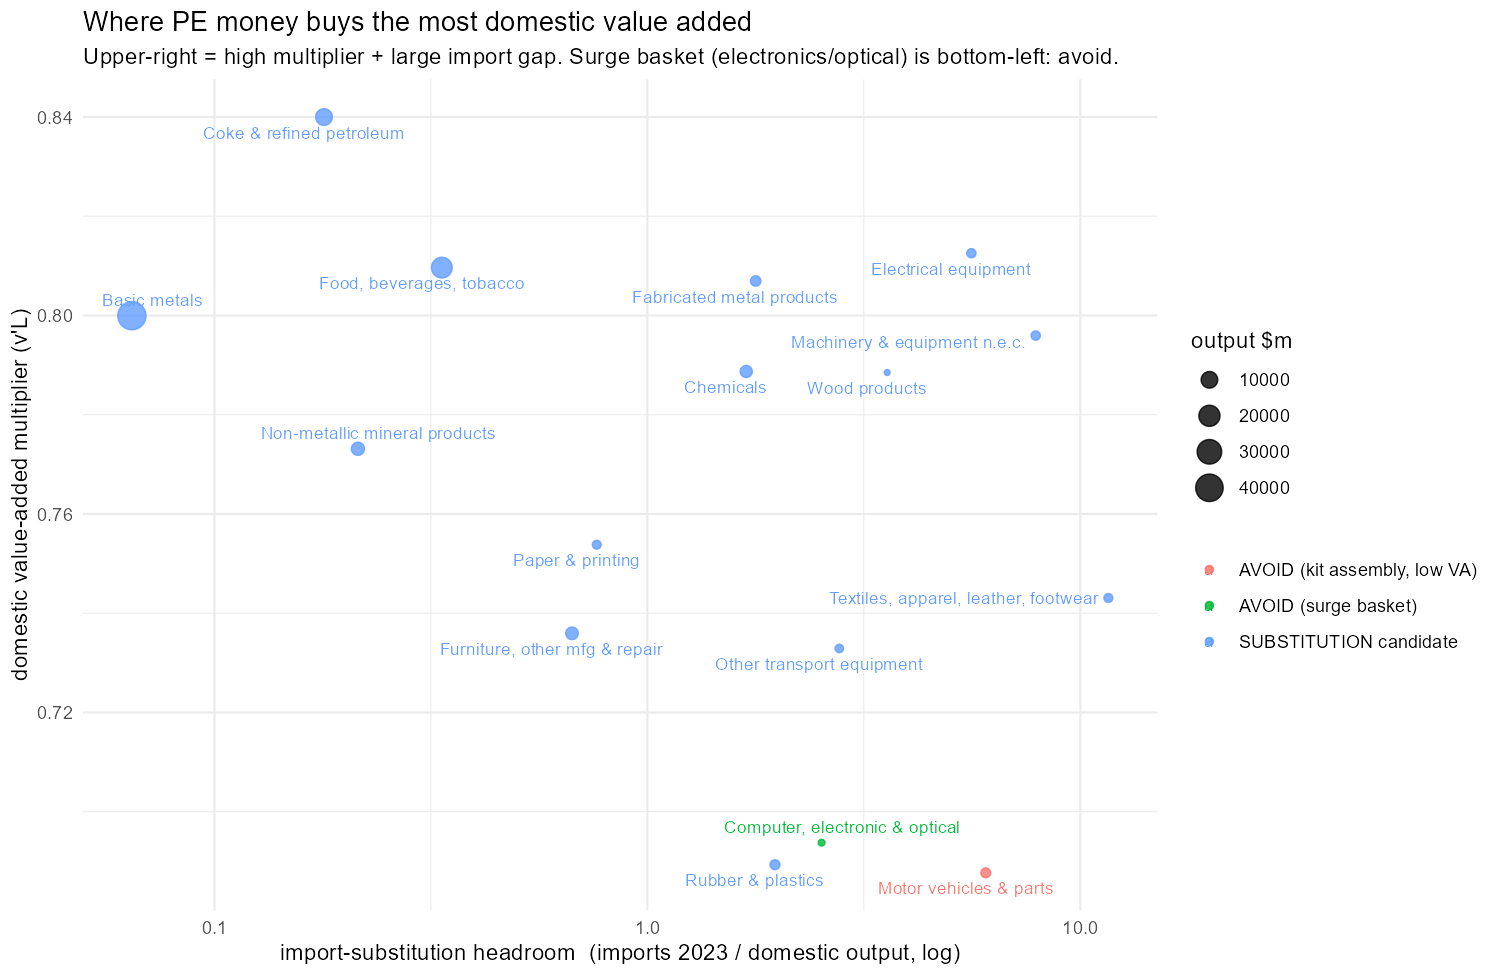
\includegraphics[width=\textwidth]{sector_priority_fig.png}
\caption{Где инвестиции покупают больше всего внутренней добавленной стоимости:
мультипликатор внутренней добавленной стоимости против запаса для импортозамещения (импорт
2023 года / внутренний выпуск, логарифмическая шкала), размер пузырька = внутренний выпуск.
Продукция корзины всплеска (компьютеры/электроника/оптика) находится внизу.}
\label{fig:priority}
\end{figure}

Эти возможности инвестиционно привлекательны в масштабе лишь в том случае, если
государственная инвестиционная корпорация сместится от роли ведущего прямого инвестора к
роли соинвестора за частными лидерами сделок, с более крупными синдицированными траншами и
надёжным выходом через листинг, а не будет полагаться лишь на приватно согласованные
продажи стратегическим инвесторам, обратные выкупы и вторичные продажи, которые сегодня
доминируют среди предпочтений выхода. Это вопрос об институтах рынка капитала, который
рассматривается в сопутствующей статье.

\section{Выводы для политики}\label{sec:policy}

Теоретическая рамка раздела~\ref{sec:framework} — это также перечень рычагов воздействия.
Шок спроса такого рода индустриализирует транзитную экономику лишь если выполняется хотя бы
одно из трёх условий: шлюз доступа к рынку закрыт для чистого реэкспорта, открыт шлюз
необратимости либо открыт институциональный шлюз. Каждое из них ниже рассматривается по
очереди применительно к Казахстану, а затем — что добавляет его положение на сухопутном
маршруте Китай--Европа и что мог бы сделать его основной поставщик. Обсуждение носит
нормативный и перспективный характер, отделено от позитивных результатов работы и опирается
на теоретическую рамку, а не на новую оценку.

\subsection{Казахстан: повышение инвестиционного отклика}

\emph{Доступ к рынку.} Таможенный союз делает торговлю почти идеальным заменителем
производства, что близко к достаточному условию нулевого отклика лишь совместно с малой
маржой трансформации, а не само по себе (раздел~\ref{sec:framework}). Соответствующий рычаг
— сделать некоторую внутреннюю добавленную стоимость условием захвата потока: правила
закупок и инвестиционного стимулирования, вознаграждающие внутреннюю переработку, и
использование позиции в таможенном союзе для привлечения именно сборки, а не только
транзита. Целью должны быть секторы замещения и платформенные секторы, а также \emph{следующий}
подобный шок, а не сами товары корзины всплеска (строки «избегать» в
Таблице~\ref{tab:priority}, где внутренняя сборка импортных комплектов даёт низкий
мультипликатор $0.69$, а принуждение к ней в основном отпугнуло бы сам поток): постоянное
правило, при котором потоки выше порога запускают проверку на местное содержание, направило
бы инвестиции к позициям с мультипликатором $0.80$ и от сборки готовых изделий с низкой
добавленной стоимостью. Это самый острый и самый трудный из рычагов. Он обменивает часть
текущего потока на шанс на устойчивые мощности, а односторонние требования к местному
содержанию применительно к \emph{транзитной} торговле плохо согласуются с правилами общего
рынка Евразийского экономического союза о свободном движении товаров
\citep{eaeu2014treaty}, поэтому реализуемая форма — это внутреннее стимулирование или
преференция при закупках либо мера, согласованная на уровне союза, а не пограничное
ограничение, которое Казахстан мог бы ввести в одностороннем порядке.

\emph{Необратимость.} Строительство мощностей выгоднее ожидания лишь тогда, когда шок
достаточно устойчив и определён, а технология достаточно дешева для невозвратных вложений.
Политика может воздействовать на два из этих трёх параметров. Она может снизить эффективную
неопределённость $\sigma$ через многолетние обязательства и надёжные сигналы спроса:
якорные контракты и контракты на закупку продукции, государственную агрегацию спроса между
министерствами и государственными компаниями и устойчивое правило о продолжительности
действия стимула. Она может снизить эффективные невозвратные издержки $I$ через совместную
пилотную и испытательную инфраструктуру, готовую к заселению аренду в специальных
экономических зонах и софинансирование первых в своём роде объектов, чтобы ни один
отдельный участник не нёс весь невозвратный риск в одиночку. Напряжение, присущее этому
рычагу, — перенос фискального риска: контракт на закупку или агрегацию спроса,
поддержанный государством, переносит риск спроса с инвестора на бюджет, и если поток
прекратится, потери ляжет на налогоплательщика, а не на фирму. С учётом волны
национализаций 2022--2025 годов, которая уже сконцентрировала промышленный риск на балансе
государства, оправданный вариант — это ограниченная по сумме, срочная и частичная гарантия,
привязанная к вехам внутренней добавленной стоимости, а не бессрочное обязательство по
закупке.

\emph{Институты.} Устойчивые смежные возможности, которые раскрывает шок (логистическая и
транспортная поддержка, импортозамещение в машиностроении и производстве металлических
изделий), финансируются лишь медленно и лишь директивным государственным капиталом. Рычаг
— сместить государственную инвестиционную корпорацию от роли ведущего прямого инвестора к
роли якорного партнёра с ограниченной ответственностью и соинвестора за независимыми
управляющими, с более крупными синдицированными траншами и надёжным маршрутом выхода через
публичный рынок: публичный листинг сегодня привлекает менее одной десятой предпочтений
выхода по данным опроса, против продаж стратегическим инвесторам, обратных выкупов и
вторичных продаж, которые вместе доминируют \citep{qicaifcifc2026pe}, а построение
внутреннего рынка выхода через прямые инвестиции параллельно с этим означает расширение
именно этого маршрута.

По всем трём рычагам первоочередным объектом инвестиций является сама логистическая
платформа (складское хозяйство, транспортная поддержка и Транскаспийские мощности): как
показано в разделе~\ref{sec:where}, она несёт наивысший мультипликатор внутренней
добавленной стоимости среди секторов-кандидатов и создаёт стоимость, которая сохраняется
независимо от того, сохранится ли какой-либо конкретный поток.

\subsection{Рычаги коридора в текущей географии}

Переговорная позиция Казахстана по этим вопросам сильнее, чем предполагают одни лишь
показатели удерживаемой стоимости. Закрытие северного наземного коридора и нарушение
основных морских маршрутов в 2023--2025 годах, описанные в разделе~\ref{sec:setting},
оставляют кратчайший наземный путь Китай--Европа, минующий и Россию, и морские узкие места,
проходящим через Казахстан и через Каспий. Казахстан близок к статусу неизбежного узла на
этом маршруте — структурного рычага в переговорах с Китаем, который заинтересован в
диверсификации и устойчивости маршрутов, и с Европейским союзом, который заинтересован в
наземном варианте, не проходящем через Россию.

Долгосрочная стратегия, в терминах теоретической рамки, состоит в использовании доступа к
коридору, мощности и гарантий надёжности как рычага, который в противном случае устраняет
таможенный союз: увязывать обязательства по пропускной способности и приоритетной обработке
с требованиями или стимулами для совместно размещённой переработки, местного содержания,
сборки по схеме совместных предприятий, а также передачи стандартов и технологий,
конвертируя транзитную ренту в мощности, создающие добавленную стоимость, а не просто
собирая сборы за чистый транзит. Это та же рекомендация, что и рычаг доступа к рынку выше,
но полученная исходя из географии, а не из правила таможенного союза.

Ценность здесь заключена в опции, а не в транзитном сборе. Транскаспийский маршрут перевёз
порядка $2$--$3$ млн тонн в 2023--2024 годах, а к 2030 году ориентирован примерно на
$10$ млн \citep{worldbank2023middlecorridor}, против товарооборота Китай--ЕС порядка
\$800 млрд в год; транзитные и обрабатывающие сборы даже при объёме 2030 года составляют
долю процента ВВП Казахстана. Значение маршрута — в том, что он является предельным
наземным звеном, которое понадобилось бы Китаю и ЕС в случае сохранения морских сбоев, и
его нынешний доход от этого не зависит.

Рычаг ограничен. Транзитный спрос оспорим: южный маршрут через Иран и Турцию и конкурирующие
каспийские узлы в Азербайджане и Грузии захватили бы часть любой ренты. Пропускная
способность каспийских паромов и портов, а также разница в ширине колеи ограничивают, сколько
трафика маршрут реально способен принять. Кроме того, преимущество сохраняется лишь до тех
пор, пока продолжаются сбои в узких местах и остаётся незавершённой диверсификация
маршрутов Китаем.

\subsection{Китай: снижение барьеров для большего захвата стоимости Казахстаном}

Поскольку Китай обеспечивает около двух третей входящего потока, часть рычагов находится на
китайской стороне. Это гипотезы, которые работа не может проверить, они предлагаются как
направления, а не как выводы. Правила возврата НДС и переработки на экспорт — важные
инструменты китайской промышленной политики, чьи ставки резко различаются по товарам и
заметно смещают структуру экспорта \citep{gourdon2022vat} — в настоящее время благоприятствуют
экспорту готовых изделий над экспортом компонентов и сборкой в Казахстане, склоняя фирмы к
отправке готового изделия, а не к размещению стадии производства на маршруте.
Административные барьеры для среднемасштабных исходящих совместных предприятий в
Центральной Азии повышают постоянные издержки создания предприятия того рода, который
добавлял бы внутреннюю стоимость. Взаимное признание стандартов и сертификации позволило бы
собранному в Казахстане товару соответствовать требованиям как китайского, так и
евразийского рынка без повторного процесса подтверждения соответствия. Координация зон
таможенной переработки в рамках Транскаспийской инициативы и «Пояса и пути» дала бы
совместно размещённой сборке тот же таможенный режим, что и чистому транзиту.

Ни один из этих рычагов не заменяет остальные: рычаги доступа к рынку и коридорного влияния
— самые мощные и самые трудные для приведения в действие, а институциональный рычаг —
необходимое условие для того, чтобы частный капитал начал действовать после того, как
приведены в действие первые два.

\section{Обсуждение}\label{sec:discussion}

Торговля Казахстана с Россией и с Западом по этим товарам изменилась на порядок величины
после 2022 года. Внутреннее экономическое содержание этого движения невелико: добавленная
стоимость составляет примерно одну десятую от промышленного эквивалента, таможенная пошлина
— менее одного процента доходов, доля процента ВВП, и никакого заметного инвестиционного
отклика. Страна функционирует как коридор, а не как площадка производства.

Результат отвечает на более общий вопрос: когда торговый шок индустриализирует страну, а
когда лишь проходит через неё транзитом? Производство — более вероятный отклик тем в
большей степени, чем меньше спрос может быть удовлетворён одной лишь торговлей (закрытый
шлюз доступа к рынку), чем более устойчив и определён шок, а технология достаточно дешева
для невозвратных вложений, так что строительство выгоднее ожидания (открытый шлюз
необратимости), и чем больше рынок капитала способен профинансировать проходящие отбор
проекты (открытый институциональный шлюз); мы рассматриваем их как три соображения,
повышающие вероятность отклика предложения, а не как условия, которые мы выводим как
совместно необходимые. Казахстанский кейс фиксирует первое условие и половину третьего:
таможенный союз делает торговлю близким заменителем производства, поэтому шок поглощается
торговым каналом, а государственная инвестиционная корпорация, не испытывающая ограничения
рынка капитала, также не стала строить, что несовместимо с институциональным шлюзом как
связывающим ограничением для этого нулевого отклика (хотя её мандат и подверженность
трансграничным комплаенс-рискам осложняют сопоставление). Связывает ли шлюз необратимости
\emph{самостоятельно} — кейс сказать не может: поскольку реэкспортный поток фактически
сохранялся вплоть до 2025 года, нулевой отклик нельзя трактовать как реакцию на
наблюдаемый временный шок; то, с чем столкнулся участник рынка в 2022 году, — это
неопределённость относительно продолжительности шока, а сопоставление устойчивого и
неопределённого шоков одновременно смещает более одного шлюза. Институциональный шлюз
объясняет упущенную альтернативу: смежные устойчивые возможности, которые раскрывает шок, в
логистике и машиностроении, остаются на попечении медленного директивного государственного
капитала и не финансируются частным капиталом, хотя их шлюз необратимости открыт. Армения и
Турция показывают тот же всплеск 2022 года (Кыргызская Республика и Грузия — на повышенном
уровне с 2022 года на более шумных рядах; Приложение~\ref{app:breaks}) и, по имеющимся у нас
данным, не имеют внутреннего сектора производства компонентов для расширения; контрастные
случаи теоретической рамки (структурные переориентации либо режимы правил происхождения,
принуждающие к внутреннему содержанию) — это случаи, где отклик предложения всё же
происходит, даже без глубокого рынка капитала. Статическая стоимость, которую упускает
Казахстан (добавленная стоимость на уровне одной десятой промышленного эквивалента), —
меньшая часть издержек; большая часть — динамическая. Режим правил происхождения или
местного содержания, который вынудил бы разместить стадию производства внутри страны, также
создал бы обратные связи, через которые иностранные поставщики передают технологии и
повышают производительность внутренних фирм \citep{javorcik2004spillovers}, а также обучение
у поставщика и диффузию, которые сопутствуют устойчивым производственным отношениям
\citep{desouza2024diffusion}. Чистый коридор упускает всё это: товары проходят транзитом, ни
разу не вовлекая внутреннюю фирму в цепочку поставок, поэтому и учиться не у кого. Именно в
этом заключена долгосрочная цена статуса коридора, и она не отражена в арифметике
добавленной стоимости.

\paragraph{Одновременный рост обрабатывающей промышленности и почему это не контрпример.}
За тот же период агрегированный сектор обрабатывающей промышленности Казахстана
действительно вырос: за январь--июль 2026 года на него пришлось около 47\% промышленного
производства против 46\% у горнодобывающей промышленности (второй год подряд, когда
обрабатывающая промышленность опережает), при этом обрабатывающая промышленность выросла
примерно на 9\% год к году, тогда как горнодобывающая упала примерно на 4\%, а добыча сырой
нефти — примерно на 9\% \citep{qazstat2026industry}. В контексте настоящей работы этот рост
согласуется с теоретической рамкой. Часть перекрёстного эффекта — в знаменателе: горная и
нефтяная отрасли сократились, поэтому растущая \emph{доля} обрабатывающей промышленности
завышает реальное расхождение. Рост сконцентрирован в производстве легковых автомобилей и
сборке (выпуск машиностроения вырос примерно на 22\%, на предприятиях полного цикла с
объявленными мощностями порядка 190~000 единиц) и в импортозамещении для внутреннего
спроса (металлические изделия, химическая продукция, фармацевтика), а не в позициях
реэкспорта данного исследования, где новых мощностей не появилось. Механизм также
соответствует тому, что называет теоретическая рамка: минимальные доли местного содержания,
прописанные в контрактах на недропользование, переход к обязательным закупкам у внутренних
производителей крупными фирмами и государственными агентствами, офтейк-контракты,
обеспечивающие спрос, и директивное государственное финансирование и финансирование
институтов развития за новыми предприятиями \citep{kzgov2026domprod,eaeu2014treaty}. Это
намеренно \emph{закрытый} шлюз доступа к рынку в сочетании с директивными институтами —
именно та конфигурация, при которой теоретическая рамка предсказывает отклик предложения.
Там, где Казахстан требовал внутреннего содержания или сам обеспечивал спрос, инвестиции
последовали; там, где товар мог беспрепятственно двигаться далее внутри таможенного союза
без трансформации, они не последовали.

\paragraph{Ограничения.} Центральными являются четыре ограничения. Во-первых, кейс наблюдает
единственную конфигурацию, в которой три шлюза не идентифицированы по отдельности. Он всё
же может зафиксировать шлюз доступа к рынку как открытый и обнаружить свидетельства,
несовместимые с институциональным шлюзом рынка капитала как связывающим ограничением для
нулевого отклика, специфичного для данного шока; чего кейс установить не может — это то,
что необратимость связывает самостоятельно. Сопоставление устойчивого и неопределённого
шоков и конвейер государственного фонда — наводящее подтверждение, а не чистые эксперименты,
а межстрановая панель, которая позволила бы разделить шлюзы необратимости и институтов,
требует отраслевых данных о гринфилд-проектах по странам. Во-вторых, заголовочный показатель
удерживаемой стоимости — это калибровка: поскольку шаг «затраты--выпуск» почти не влияет на
результат, он масштабируется пропорционально торговой марже, которую мы выбираем, а не
оцениваем (раздел~\ref{sec:capture}); интерпретация «коридор, а не завод» (переориентированный
доллар стоит около одной десятой произведённого) сохраняется при марже вплоть до примерно
одной восьмой, ослабевая до «около одной пятой» при марже около одной пятой. В-третьих,
инвестиционный нулевой отклик \emph{переопределён}, поскольку беспорядки января 2022 года,
трансграничные комплаенс-риски, отмеченные в разделе~\ref{sec:setting}, и волна
национализаций каждый по отдельности снижали бы число сделок, поэтому мы ограничиваем его
масштаб (раздел~\ref{sec:investment}), а не приписываем его исключительно торговому шоку.
В-четвёртых, базы данных о сделках фиксируют \emph{транзакционные} инвестиции (M\&A и
раунды частного финансирования) и недостаточно охватывают чистые гринфилд-мощности,
созданные без внешней транзакции, а также ограничены только Казахстаном, поэтому мы не
можем использовать их для проверки предсказания теоретической рамки о том, что посредники
вне ЕАЭС (Турция, Грузия) должны с большей вероятностью показать отклик в форме переработки.
Специализированный реестр гринфилд-инвестиций (fDi Markets либо Orbis Cross-Border
Investment) закрыл бы оба пробела; свидетельства на уровне заводов, которые мы используем в
разделе~\ref{sec:why}, и поиски публичных источников в разделах~\ref{sec:why}
и~\ref{sec:moderators} по мощностям сектора компонентов в Казахстане и по дифференцированному
отклику в Турции и Грузии — это ручные заменители, более слабые инструменты, чем покупной
реестр. Эти два поиска — не свидетельство одного и того же рода: поиск по компонентам в
Казахстане не выявляет мощностей там, где теоретическая рамка не предсказывает их, что
согласуется с рамкой; поиск по Турции/Грузии не выявляет дифференцированного отклика там,
где рамка предсказывает, что он \emph{должен} появиться у посредников вне ЕАЭС, что
представляет собой нулевой результат при слабом инструменте, который не находит
предсказанного различия и потому не подтверждает предсказание, а не согласуется с ним.
Межстрановое предсказание остаётся непроверенным на том же уровне строгости, который работа
предъявляет к себе в остальном.

Ряд решений по измерению также влияет на оценки. Входящая сторона — это данные,
отражённые в отчётности партнёров (зеркальные), которые завышают казахстанское поглощение
для товаров, движущихся далее. Во входящем потоке доминирует крупная, уже существовавшая
компонента Китая, поэтому мы измеряем удерживаемую стоимость на приростном западном потоке
и учитываем входящий поток «Запад + Китай» лишь на уровне товарных позиций, где
фиксированные эффекты позиции и года поглощают китайский тренд. Корзина всплеска отобрана
по результату после 2022 года; составленный извне приоритетный список переламывается в ту
же дату, и его значимый коэффициент несётся существенно, хотя и не полностью, 24 позициями,
которые он разделяет с корзиной всплеска, — 26 позиций, которые он не разделяет, при
сопоставлении с контрольной группой, очищенной от корзины всплеска, независимо значимы по
исходящему потоку, но с меньшей величиной (Таблица~\ref{tab:did}), поэтому это частичное,
менее масштабное подтверждение, а не полностью независимое воспроизведение. Поэтому мы
трактуем кросс-секционную разность разностей наряду со структурными переломами и
сопоставлением с соседними странами, а не самостоятельно, а плацебо на крупнейших
гражданских позициях значимо с противоположным знаком, что указывает на неоднородность
контрольной группы по тренду. Удерживаемая маржа взята из конвенции национальных счетов
(6--14\%), а не оценена построчно, а мультипликаторы добавленной стоимости получены из
OECD ICIO (2019 год), перекрёстно проверены по национальной таблице «затраты--выпуск»
Казахстана (2023 год) с тем же качественным результатом.

\appendix
\renewcommand{\thesection}{\Alph{section}}
\numberwithin{table}{section}
\numberwithin{figure}{section}

\section{Спецификация запроса к базе данных сделок}\label{app:deals}
\emph{Для онлайн-публикации.}

\medskip
Казахстанская выборка сделок извлечена из трёх коммерческих баз данных (Capital~IQ,
PitchBook, Preqin). Общие параметры: \emph{география цели/эмитента} = Казахстан (страна
регистрации либо основной деятельности); \emph{дата объявления} — между 1~января 2015 года
и 31~декабря 2025 года; \emph{типы сделок} = слияние/поглощение, мажоритарная/миноритарная
доля, выкуп и сделки роста прямых инвестиций, венчур (все стадии), совместное предприятие и
PIPE/частное размещение; \emph{статус} = завершена или объявлена (ожидающие и отозванные
сделки фиксируются отдельно). Финансовые показатели — в долл. США на дату объявления.

\begin{description}
\item[Capital~IQ (S\&P):] Screening $>$ Transactions; местоположение целевой компании =
Казахстан; типы транзакций как указано выше; диапазон дат объявления как указано выше.
Экспорт всех столбцов; дата выгрузки зафиксирована в файле для воспроизведения результатов.
\item[PitchBook:] Advanced Search $>$ Deals; местоположение штаб-квартиры компании =
Казахстан; типы сделок = M\&A, Buyout\slash LBO, PE Growth\slash Expansion, все стадии VC,
Angel, Accelerator\slash Incubator; диапазон дат сделки как указано выше.
\item[Preqin:] Private Equity $>$ Deals \& Exits; страна портфельной компании = Казахстан;
диапазон дат сделки как указано выше.
\end{description}

Устранение дублей проводится по названию цели, дате объявления ($\pm$30 дней) и типу
сделки. Отраслевая классификация приведена к отраслям ISIC ред.~4 из нативной таксономии
каждой базы данных через документированную таблицу соответствия. Три выборки, таблица
соответствия и скрипт сверки приведены в пакете для воспроизведения результатов, который
фиксирует дату выгрузки каждого источника и его самый ранний год достаточно полного охвата
Казахстана.

\section{Построение набора товаров}\label{app:products}
\emph{Для онлайн-публикации.}

\medskip
Набор кандидатов состоит из 75 позиций HS6: 50 — из внешне составленного перечня
технологически ёмких позиций, опубликованного в феврале 2024 года («приоритетный список»),
сгруппированных издателем в шесть уровней, плюс 25 однозначно гражданских контрольных
позиций. \textbf{Корзина всплеска} определяется по данным как позиции, по которым средний
входящий поток (западные страны-респонденты + Китай) и средний отток в Россию \emph{каждый}
как минимум удвоились с 2019--2021 годов по 2022--2024 годы, при этом отношение вычислено
после добавления \$10~000 к числителю и знаменателю, с постпериодными порогами \$0.2 млн
(входящий поток) и \$0.1 млн (исходящий). Отбор проходят двадцать девять позиций; 24 из них
входят в приоритетный список, а 5 — контрольные позиции, которые также показали всплеск. Из
75 кандидатов 55 проходят удвоение по исходящему потоку и 41 — по входящему; требование
выполнения обоих условий и является связывающим фильтром.

\begin{table}[htbp]
\centering
\caption{Коды HS6 приоритетного списка по уровням издателя и гражданский контрольный
набор. $\dagger$ отмечает 29 позиций корзины всплеска.}
\label{tab:appb}
\footnotesize
\begin{tabular}{@{}p{1.6cm}p{12.4cm}@{}}
\toprule
Уровень & Коды HS6 \\
\midrule
1 & 854231$\dagger$, 854232, 854233$\dagger$, 854239$\dagger$ \\
2 & 851762$\dagger$, 852691$\dagger$, 853221, 853224, 854800$\dagger$ \\
3A & 847150, 850440, 851769, 852589$\dagger$, 852910, 852990, 853669$\dagger$, 853690, 854110$\dagger$, 854121, 854129$\dagger$, 854130, 854149$\dagger$, 854151, 854159$\dagger$, 854160 \\
3B & 848210, 848220$\dagger$, 848230$\dagger$, 848250, 880730, 901310$\dagger$, 901380, 901420, 901480 \\
4A & 847180$\dagger$, 848610, 848620, 848640, 853400, 854320$\dagger$, 902750$\dagger$, 903020, 903032$\dagger$, 903039$\dagger$, 903082 \\
4B & 845710$\dagger$, 845811$\dagger$, 845891$\dagger$, 845961, 846693$\dagger$ \\
\midrule
Контроль & 090111, 170490, 190590, 210390, 210690, 220300, 330300, 330499, 340111, 392321, 392490$\dagger$, 401110$\dagger$, 480256, 610910$\dagger$, 611020$\dagger$, 620342, 630260, 640399, 691110, 732690, 841810, 870899, 940360, 950300, 961900$\dagger$ \\
\bottomrule
\end{tabular}

\vspace{2pt}
\footnotesize Приоритетный список: List of Common High Priority Items ЕС/США/Великобритании/Японии,
версия от февраля 2024 года. Обозначения уровней принадлежат издателю; мы сохраняем их без
изменений.
\end{table}

\section{Устойчивость разности разностей}\label{app:did}
\emph{Для онлайн-публикации.}

\medskip
Таблица~\ref{tab:appc} собирает полную батарею проверок, изложенную в
разделе~\ref{sec:did}. Результирующим показателем повсюду выступает $\text{asinh}$ от
экспорта Казахстана в Россию; $\gamma$ — коэффициент при
$\text{лечение}\times\text{после}$ с фиксированными эффектами HS6 и года и устойчивыми к
кластеризации стандартными ошибками по HS6, если не указано иное.

\begin{table}[htbp]
\centering
\caption{Устойчивость разности разностей, корзина всплеска, экспорт в Россию. Фиктивное
«лечение» плацебо присвоено шести крупнейшим гражданским позициям по размеру до 2022 года;
ни одна из шести не входит в корзину всплеска.}
\label{tab:appc}
\footnotesize
\begin{tabular}{@{}lrrr@{}}
\toprule
Спецификация & $\gamma$ & ст. ош. & $p$ \\
\midrule
Базовая (ФЭ HS6 + год)                              & 2.44 & 0.96 & 0.013 \\
\quad wild-cluster-бутстрап $p$ (B $=$ 1999)          &      &      & 0.010 \\
\quad скорректировано по Холму по 4 результатам корзины &      &      & 0.039 \\
$+$ ФЭ дециль размера $\times$ год                       & 2.29 &      & 0.003 \\
Полное исключение 2022 года                                    & 2.71 & 1.05 & 0.012 \\
Донат (искл. 2022, год «лечения» $=$ 2023)             & 2.71 & 1.05 & 0.012 \\
Пуассон (PPML) в уровнях, $e^{\beta}$                  & 3.5$\times$ &      & 0.020 \\
Приоритетный список (50 HS6, внешний)             & 2.88 & 0.74 & $<0.001$ \\
\quad из них 26 позиций, vs.\ очищ. гражд. контроль ($N=368$) & 1.94 & 0.90 & 0.037 \\
\quad\quad wild-cluster-бутстрап $p$ (B $=$ 1999)      &      &      & 0.035 \\
\quad\quad совместный предтрендовый тест Вальда ($F$, 3 и 45 DoF)     & 0.75 &      & 0.528 \\
Коэфф. анализа событий 2018 года (вне окна отбора) & 0.19 & 0.90 & 0.835 \\
Плацебо (крупнейшие гражданские позиции)                       & $-0.95$ & 0.25 & 0.001 \\
\midrule
\multicolumn{4}{@{}l}{\emph{Джекнайф с последовательным исключением группы HS2}} \\
Искл. HS 39 (1 позиция)                                   & 2.51 & 0.98 & 0.013 \\
Искл. HS 40 (1 позиция)                                   & 2.48 & 0.98 & 0.014 \\
Искл. HS 61 (2 позиции)                                  & 2.67 & 1.00 & 0.009 \\
Искл. HS 84 (7 позиций)                                  & 2.28 & 1.18 & 0.058 \\
Искл. HS 85 (13 позиций)                                 & 1.36 & 1.06 & 0.207 \\
Искл. HS 90 (4 позиции)                                  & 3.16 & 0.96 & 0.002 \\
Искл. HS 96 (1 позиция)                                   & 2.59 & 0.97 & 0.010 \\
\midrule
\multicolumn{4}{@{}l}{\emph{Альтернативные пороги отбора корзины всплеска (по обоим плечам)}} \\
$1.5\times$ (40 позиций)                                & 1.59 & 0.90 & 0.080 \\
$2.0\times$ (29 позиций, базовый)                      & 2.44 & 0.96 & 0.013 \\
$2.5\times$ (23 позиции)                                & 3.12 & 1.08 & 0.005 \\
$3.0\times$ (18 позиций)                                & 3.16 & 1.27 & 0.015 \\
\midrule
\multicolumn{4}{@{}l}{\emph{Рандомизационный вывод, согласованный с правилом отбора}} \\
\multicolumn{4}{@{}p{15.3cm}}{\footnotesize Свободная перестановка (годовые метки внутри
HS6, правило применено повторно): правило отбирает в среднем 5.0 позиций при $H_0$
(максимум 12 из 1{,}000 розыгрышей), поэтому
$P(\text{правило отбирает}\ge 29\mid H_0)=0.000$; нулевое распределение перестановки для
$\gamma$ имеет среднее 2.79, ст. откл.\ 1.50, 95-й перцентиль 5.37, и
$P(|\gamma^{\text{perm}}|\ge 2.44)=0.58$.} \\
\multicolumn{4}{@{}p{15.3cm}}{\footnotesize Сохраняющий тренд циклический сдвиг: в среднем
отобрано 5.2 позиции (максимум 19), $P(\ge 29\mid H_0)=0.000$; нулевое распределение
$\gamma$ при циклическом сдвиге (который сохраняет собственный тренд и автокорреляцию
каждой позиции, в отличие от свободной перестановки) имеет среднее 1.64, ст. откл.\ 1.20, и
$P(|\gamma^{\text{cyc}}|\ge 2.44)=0.29$ --- уже, чем при свободной перестановке, как и
ожидалось, но не опровергает вывод о том, что величина эффекта не отделима от отбора.} \\
\multicolumn{4}{@{}p{15.3cm}}{\footnotesize Приоритетный список: случайная корзина из 50
позиций, выбранных из всех позиций HS6, которые Казахстан экспортирует в Россию, имеет
нулевое распределение $\gamma$ со средним 0.00, ст. откл.\ 0.97, и
$P(|\gamma^{\text{perm}}|\ge 2.88)=0.002$ --- согласуется с тем, что коэффициент
приоритетного списка несётся его действительно затронутым «лечением» пересечением с
корзиной всплеска (Таблица~\ref{tab:did}), а не является артефактом случайного выбора 50
позиций.} \\
\bottomrule
\end{tabular}
\end{table}

\section{Удерживаемая стоимость: детализация «затраты--выпуск»}\label{app:io}
\emph{Для онлайн-публикации.}

\medskip
Внутренняя добавленная стоимость на переориентированный доллар равна $m\,\bar v^{TT}$,
против $\bar v^{M}$ на доллар внутреннего промышленного производства. По блоку Казахстана
OECD ICIO $\bar v^{TT} = 0.787$ (торговля, транспорт, складское хозяйство) и
$\bar v^{M} = 0.764$ (обрабатывающая промышленность), поэтому отношение
переориентированного к произведённому составляет $\approx 1.03\,m$, а шаг
«затраты--выпуск» почти не выполняет никакой работы. Пересчёт по симметричной таблице
«затраты--выпуск» Бюро национальной статистики Казахстана (2023 год, сопоставлено 57
отраслей, взвешено по выпуску внутри группы) даёт $\bar v^{TT} = 0.885$ и
$\bar v^{M} = 0.742$, смещая отношение с $0.10$ до $0.12$. Таблица ресурсов Бюро
национальной статистики задаёт границы для $m$: чисто транспортная маржа для машин и
электроники составляет около $1\%$ стоимости в базовых ценах, а полная торгово-транспортная
маржа (которая несёт розничное звено, которое коридор никогда не выполняет) — около $49\%$;
компонента торговой маржи сама по себе (без транспорта) составляет $48\%$ для той же
категории, подтверждая, что транспорт — малая часть полной маржи здесь, хотя таблица не
разделяет опт и розницу и потому не может самостоятельно подтвердить чисто оптовую
интерпретацию. Диапазон 6--14\% — это оптово-транспортная интерпретация, выше пола и
значительно ниже потолка; ниже показано, как это соотносится с оценкой $0.34$ по
сопоставленным ячейкам.

\begin{table}[htbp]
\centering
\caption{Чувствительность заголовочного показателя удерживаемой стоимости к удерживаемой
марже $m$. Отношение $=$ внутренняя добавленная стоимость на переориентированный доллар,
относительно произведённого доллара ($m\,\bar v^{TT}/\bar v^{M}$, OECD ICIO).}
\label{tab:appd}
\footnotesize
\begin{tabular}{@{}lrrrr@{}}
\toprule
$m$ & 0.06 & 0.10 & 0.14 & 0.19 \\
\midrule
ВДС на переориент. \$ & 0.047 & 0.079 & 0.110 & 0.150 \\
Отношение к произвед. \$ & 0.062 & 0.103 & 0.144 & 0.196 \\
Удержано, \$ млн (из \$479 млн) & 23 & 38 & 53 & 72 \\
\midrule
$m$ & 0.25 & 0.32 & 0.34 & 0.49 \\
\midrule
ВДС на переориент. \$ & 0.197 & 0.252 & 0.268 & 0.386 \\
Отношение к произвед. \$ & 0.258 & 0.330 & 0.350 & 0.505 \\
Удержано, \$ млн (из \$479 млн) & 94 & 121 & 128 & 185 \\
\bottomrule
\end{tabular}

\vspace{2pt}
\footnotesize Ориентиры: чисто транспортная $m\approx 0.01$; оптово-транспортный диапазон
$0.06$--$0.14$; цензурированная валовая маржа по сопоставленным ячейкам $0.34$; полная
торгово-транспортная маржа $0.49$. Интерпретация «коридор, а не завод» (переориентированный
доллар $\approx$ одной десятой произведённого) сохраняется при $m$ вплоть до примерно
$0.12$; она ослабевает до «около одной пятой» при $m\approx 0.19$, «около трети» при
$m\approx 0.32$ и примерно до половины при $m\approx 0.49$.
\end{table}

Мы не полностью согласуем цензурированную валовую маржу по сопоставленным ячейкам ($0.34$)
с диапазоном $6$--$14\%$. Занижение декларирования исходящего экспорта, которое
потребовалось бы для объяснения показателя в одну пятую внутренней стоимости от валового
переориентированного потока, составляет $13$--$21\%$ (раздел~\ref{sec:capture}); эта
граница сама по себе недостаточно велика, чтобы снизить $0.34$ до нашего диапазона, поэтому
по крайней мере часть разрыва, вероятно, отражает несовпадение базы c.i.f./f.o.b., а не
только занижение декларирования. Мы не можем разделить эти два компонента на имеющихся
данных и рассматриваем $0.34$ как верхнюю границу, которую должен выдержать качественный
вывод работы (Таблица~\ref{tab:appd} показывает, что выдерживает — на уровне «около трети»),
а не как подтверждённую точечную оценку $m$.

Свидетельства по удельной стоимости на уровне сопоставленных ячеек (годовые данные,
$n = 112$ ячеек HS6$\times$период) носят исключительно описательный характер. Медианное
отношение реэкспорт/импорт составляет $0.73$ на базе c.i.f./f.o.b. и $1.6$ на базе,
сопоставимой напрямую по f.o.b.; гражданская контрольная корзина даёт $0.59$ и $0.94$.
Наклон сквозного прохода $\log(\text{цена}_{\text{expRU}})$ по $\log(\text{цена}_{\text{mirWC}})$
составляет $0.48$ ($p = 0.03$), и $0.20$ ($p = 0.46$) против заявленной казахстанской
импортной цены. Наценка f.o.b. по уровням списка составляет $0.47$ (Уровень 1), $3.83$ (2),
$1.82$ (3A), $1.09$ (3B), $3.94$ (4A), $1.35$ (4B), против $1.33$ для контрольной корзины:
наценка неравномерна по уровням, а её высокие значения приходятся примерно на половину
сопоставленного валового потока — паттерн наценки за дефицит, а не равномерной маржи
переработки. Весовое отношение на уровне ячейки (реэкспортированный тоннаж к
импортированному) имеет медиану $0.08$ и агрегат $0.11$; агрегированное весовое отношение
равно агрегированному сквозному проходу стоимости ($0.11$), поэтому весовое отношение ниже
единицы — в значительной степени факт сквозного прохода. Одиннадцать процентов ячеек
превышают $1.05$, при межквартильном размахе от $0.02$ до $0.49$. В шести ячейках, близких к
чистому транзиту (сквозной проход стоимости в диапазоне $[0.8, 1.25]$), весовое отношение
составляет $0.74$ по медиане ($0.26$ и $0.94$ по квартилям).

\section{Структурные переломы у соседей и стран сопоставления}\label{app:breaks}
\emph{Для онлайн-публикации.}

\medskip
Таблица~\ref{tab:appe} приводит экспорт по корзине всплеска в Россию для других
пост-2022-х посредников и тест на смещение среднего (sup-$F$) на годовом ряде $\text{asinh}$
за $2018$--$2025$ годы. Армения и Кыргызская Республика входят в Евразийский экономический
союз с Россией; Грузия и Турция направляют товары через таможенную границу. Беларусь также
входит в Евразийский экономический союз и в популяцию посредников, но прекратила отчётность
в UN Comtrade в 2022 году, поэтому пост-2022-й ряд недоступен, и она исключена из таблицы.
Перелом 2022 года проявляется независимо от статуса таможенного союза; шок спроса
обобщается на всю популяцию, тогда как тест на инвестиции ограничен Казахстаном за
отсутствием данных о сделках в других странах. Устойчивость, однако, не обобщается: поток
Турции достигает пика в 2023 году на уровне \$207 млн и снижается до \$73 млн к 2025 году —
паттерн отката, схожий с Арменией и Кыргызской Республикой, а не с устойчивым уровнем
Казахстана в \$119--145 млн; Казахстан — единственный посредник в таблице, чей
пост-2022-й уровень не откатывается к своей траектории до 2022 года.

\begin{table}[htbp]
\centering
\caption{Экспорт по корзине всплеска в Россию, млн долл. США в год, и годовой тест на
перелом.}
\label{tab:appe}
\footnotesize
\setlength{\tabcolsep}{3.2pt}
\begin{tabular}{@{}lrrrrrrrrrrc@{}}
\toprule
& 2018 & 2019 & 2020 & 2021 & 2022 & 2023 & 2024 & 2025 & sup-$F$ & $p$ & год скачка \\
\midrule
Казахстан (ЕАЭС)        & 17 & 12 & 7 & 8 & 128 & 145 & 119 & 133 & 150.7 & $<0.001$ & 2022 \\
Армения (ЕАЭС)           & 15 & 9 & 7 & 9 & 71 & 93 & 42 & 13 & 10.5 & 0.015 & 2022 \\
Кыргызская Республика (ЕАЭС)   & 1 & 3 & 6 & 7 & 12 & 30 & 12 & 12 & 13.4 & 0.004 & 2019 \\
Турция (вне ЕАЭС)     & 53 & 55 & 47 & 58 & 119 & 207 & 98 & 73 & 11.9 & 0.007 & 2022 \\
Грузия (вне ЕАЭС)       & 0.2 & 0.7 & 0.4 & 0.7 & 1.0 & 1.1 & 1.7 & 0.7 & 6.9 & 0.075 & 2019 \\
\bottomrule
\end{tabular}

\vspace{2pt}
\footnotesize Строка Казахстана — из Таблицы~\ref{tab:magnitudes}. sup-$F$ — тест на
смещение среднего для устойчивого ряда; мы трактуем его как свидетельство наличия перелома,
а не как кардинальную величину, и он сам по себе не датирует перелом. «Год скачка» — год с
наибольшим годовым изменением $\text{asinh}$(экспорта); это зашумлённый показатель при
столь малых, от однозначных до низких двузначных, уровнях, и для Кыргызской Республики и
Грузии он приходится на 2019 год, а не на 2022-й, несмотря на то что уровни 2022 года у
обеих стран также выросли относительно среднего за 2018--2021 годы (обзор JIE, раунд 2,
рецензент B, замечание N3). Мы трактуем как свидетельство общего сбоя именно отклонение
sup-$F$, а не единственный наибольший скачок; формулировку «тот же перелом 2022 года» в
остальной части статьи лучше понимать как строго верную для Армении и Турции и как
«повышенный уровень с 2022 года», а не датированный перелом, для Кыргызской Республики и
Грузии, чьи ряды короче и более шумны. Мы предприняли попытку HAC-коррекции (Ньюи--Уэста)
теста sup-$F$ для каждой страны; на этих 8-летних годовых рядах коррекция оказалась
численно неустойчивой (выбор ширины окна сам по себе ненадёжен при таком размере выборки),
в отличие от $\sim$70-наблюдательного месячного ряда в разделе~\ref{sec:shock}, где она
является решающей и оставляет доверительный интервал практически неизменным.
\end{table}

\section{Протоколы поиска по публичным источникам}\label{app:search}
\emph{Для онлайн-публикации.}

\medskip
Два поиска по публичным источникам упоминаются в разделах~\ref{sec:investment}
и~\ref{sec:moderators} как менее надёжные заменители покупного реестра
гринфилд-инвестиций (fDi Markets или Orbis Cross-Border Investment), недоступного для
данного проекта. Оба использовали один и тот же метод: общий веб-поиск и агрегация новостей
по объявлениям о мощностях (открытие заводов, сборочные линии, расширение производственных
мощностей) в указанном секторе и окне, перепроверенные по базам данных о сделках из
раздела~\ref{sec:data} там, где сделка существовала. Ни один из поисков не использовал
покупную службу мониторинга прессы или систематический обзор отраслевых справочников,
поэтому оба являются более слабыми инструментами, чем триангуляция по автомобильному
сектору в разделе~\ref{sec:investment}, которая опиралась на более обширную публичную
отчётность именно по этому сектору.

\begin{itemize}
\item \textbf{Поиск по компонентам в Казахстане} (раздел~\ref{sec:investment}): окно
2022--2025 годов; секторы — электротехническое машиностроение, компоненты и приборостроение
(категории, смежные с корзиной всплеска); поиск проведён в сентябре 2026 года методом
общего веб-поиска по объявлениям о новых мощностях. Результат: не найдено ни одного
названного проекта новых мощностей; общая отчётность по сектору описывает лишь рост рынка и
объёмы импорта.
\item \textbf{Поиск по компонентам в Турции/Грузии} (раздел~\ref{sec:moderators}): то же
окно и те же определения секторов, применённые к Турции и Грузии; поиск проведён в сентябре
2026 года. Результат: сопоставимого проекта не найдено ни в одной из стран. Как указано в
разделе~\ref{sec:moderators}, это трактуется как неинформативный нулевой результат при
слабом инструменте для межстранового предсказания теоретической рамки, а не как его
подтверждение.
\end{itemize}

Ни один из поисков не был предварительно зарегистрирован или независимо воспроизведён; оба
раскрываются как заменители, основанные на добросовестных усилиях, а не как систематический
аудит литературы или прессы.

\section*{Декларация конфликта интересов}
Автор работает в Международном финансовом центре «Астана» (AIFC), который управляет
Международной биржей «Астана» и институционально связан с государственными
инвестиционными структурами Казахстана, а ранее сотрудничал с консалтинговой командой в
рамках проекта по торговой стратегии Казахстана. Используемые здесь показатели
инвестиционной деятельности государственного фонда взяты из отчёта, опубликованного
совместно AIFC с Qazaqstan Investment Corporation (QIC) и International Finance Corporation
(IFC). Ни одна из этих ролей не входит в эмпирический анализ, который опирается на
публичные данные и на коммерческие базы данных сделок, доступные по академической
лицензии; рекомендации для политики в разделе~\ref{sec:policy} — личная позиция автора и не
представляют AIFC, QIC или IFC.

\section*{Финансирование}
Настоящее исследование не получало специального гранта ни от одного финансирующего
агентства в государственном, коммерческом или некоммерческом секторах.

\section*{Доступность данных}
Торговый анализ использует публичные данные: UN Comtrade (годовые и месячные данные HS6),
показатели мирового развития Всемирного банка, межстрановые таблицы «затраты--выпуск» ОЭСР
(издание 2023 года) и симметричную таблицу «затраты--выпуск» и таблицу ресурсов Бюро
национальной статистики Казахстана. Данные на уровне сделок лицензированы у Capital~IQ,
PitchBook и Preqin и не подлежат распространению, но полная спецификация запроса
(Приложение~\ref{app:deals}) и нативные идентификаторы сделок из источников приведены в
пакете для воспроизведения результатов, поэтому выборка воспроизводима держателем лицензии.
Агрегированные показатели инвестиций государственного фонда взяты из опубликованного отчёта
QIC/AIFC/IFC. Код и спецификации запросов приведены в пакете для воспроизведения
результатов, в \texttt{scripts/R/}\allowbreak\texttt{kz\_passthrough/} и
\texttt{scripts/R/}\allowbreak\texttt{kz\_valueadd/}.

\section*{Декларация об использовании генеративного ИИ в процессе написания}
При подготовке данной работы автор использовал Claude (Anthropic) для составления и
редактирования текста, для помощи в написании и отладке кода анализа, а также для
структурированной внутренней проверки рукописи. Все решения по данным, аналитические
решения, результаты и интерпретации принадлежат автору; автор проверил и отредактировал
весь полученный материал и несёт полную ответственность за содержание публикации.

\section*{Заявление о вкладе авторов (CRediT)}
\textbf{Жанболат Какишев:} концептуализация, методология, программное обеспечение,
формальный анализ, курирование данных, написание — черновой вариант, написание — обзор и
редактирование, визуализация.

% abbrvnat: стиль author-date natbib, совместим с компиляцией везде, согласован с \citep/\citet.
\bibliographystyle{abbrvnat}
\bibliography{corridor}

\end{document}
</content>
